\documentclass{beamer}
\mode<presentation>
{
	\usetheme{ldv}
	\setbeamercovered{transparent}
}

% Uncomment this if you're giving a presentation in german...
%\usepackage[ngerman]{babel}

% ...and rename this to "Folie"
\newcommand{\slidenomenclature}{Slide}


\usepackage[utf8]{inputenc}
\usepackage{amsmath,amssymb,amsfonts}
\usepackage{times}
\usepackage{graphicx}
\usepackage{fancyvrb}
\usepackage{array}
\usepackage{colortbl}
\usepackage{tabularx}

% Uncomment me when you need to insert code
\usepackage{color}
\usepackage{listings}
% End Code

% Uncomment me when you need video or sound
\usepackage{multimedia}
\usepackage{hyperref}
% End video

% Header
\newcommand{\zwischentitel}{Development of Recommender Systems with a Focus on Improving User Satisfaction}
\newcommand{\leitthema}{Ozan Pekmezci}
% End Header

% Titlepage
\title{Development of Recommender Systems with a Focus on Improving User Satisfaction
}
\author{Ozan Pekmezci}
\newcommand{\presdatum}{June 2019}
\institute
{
  Lehrstuhl für Datenverarbeitung\\
}
\subtitle{Entwicklung von Empfehlungssystemen mit dem Schwerpunkt auf der Verbesserung der Benutzerzufriedenheit}
% End Titlepage


% Slides
\begin{document}

% 1. Slide: Titlepage
\begin{frame}
	\titlepage
\end{frame}

% 2. Slide: TOC
\begin{frame}
   \frametitle{Table of contents}
   \tableofcontents[subsectionstyle=hide]
\end{frame} 

% Further Slides
\section{Introduction} 
\begin{frame}
   \frametitle{What are Recommender Systems?} 
    \begin{block}{Recommender Systems(RS)}
   	Software tools and techniques that provide suggestions for items that are most likely to interest a particular user
   \end{block}
   \begin{itemize}
	\item History goes back to mid 1990's
	\item Became mainstream with e-commerce
	\item Problem: Users overloaded with information
	\item Solution: RS as a way to filter information for users
\end{itemize} 

\end{frame}

%for news, unidirectional. for job bidirectional


\subsection{Problem}
\begin{frame} 
\frametitle{Problem} 
	Aim of developers and researchers:
   \begin{itemize}
   	\item Increase interaction
   	\item Increase coverage
   	\item Increase user satisfaction
   \end{itemize} 
	Evaluation metrics and properties used:
\begin{itemize}
	\item Accuracy
\end{itemize} 
   \begin{alertblock}{Problem}
	User satisfaction may also depend on other properties such as privacy, data security, diversity, serendipity, labeling and presentation.
\end{alertblock}
\end{frame}
%Interaction: items sold

\subsection{Motivation}
\begin{frame} 
\frametitle{Motivation} 
Find answers to these questions:
\begin{itemize}
	\item Does high accuracy guarantee high user satisfaction?
	\item Does diversity affect user satisfaction positively?
	\item Would a feedback loop enhance user satisfaction?
\end{itemize} 
    \begin{block}{Use-case}
    	Individual and group recommendation of talents to roles or projects.  
\end{block}
\end{frame}

\section{Review of Literature and Research}
\begin{frame} 
\frametitle{Types of Recommender Systems} 
Two main categories:
\begin{itemize}
	\item Personalized
	\item Non-personalized
\end{itemize} 
Among personalized approaches are:
\begin{itemize}
	\item Content-based filtering
	\item Collaborative filtering
	\item Knowledge-based filtering
	\item Hybrid methods
\end{itemize} 
   \begin{alertblock}{Solution}
	Only used content-based filtering in this thesis. 
\end{alertblock}
\end{frame}

\subsection{Overview of Content-Based Recommender Systems}
\begin{frame}[plain]
\frametitle{Overview of Content-Based Recommender Systems} 
\begin{figure}
	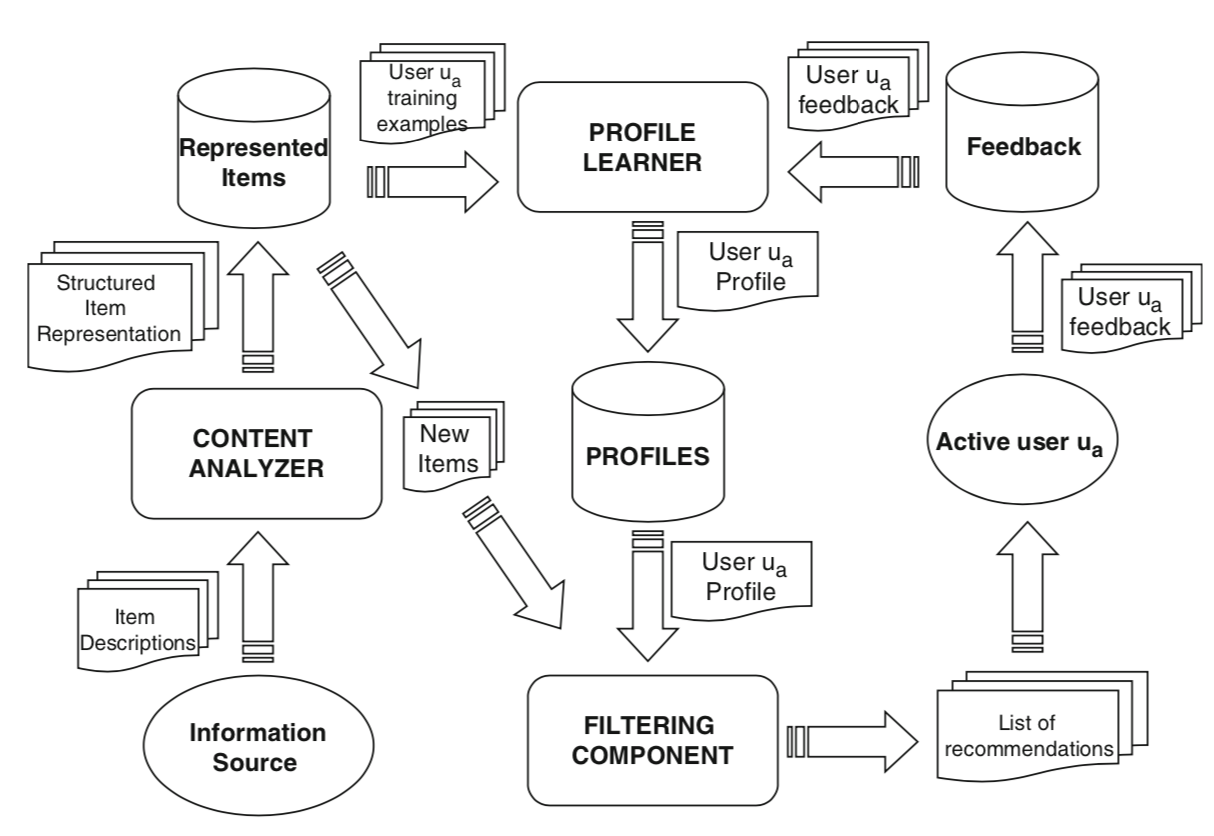
\includegraphics[scale=0.5]{images/HighLevelContentBased} 
	\caption{High level architecture of a content-based recommender}
\end{figure}
\end{frame}

% Implicit and explicit feedback

\subsection{Advantages and Drawbacks of Content-Based Filtering}
\begin{frame} 
\frametitle{Advantages and Drawbacks of Content-Based Filtering} 
Advantages:
\begin{itemize}
	\item User Independence
	\item Transparency
	\item New Item
\end{itemize} 
Drawbacks:
\begin{itemize}
	\item Limited Content Analysis
	\item Over-specialization
	\item New User
\end{itemize} 
\end{frame}

%UI: collaborative'de tum userlarin profili lazim nearest neighbor yapmak icin
%New Item: cold start problem yok

%LCA: monty python and python
% OS If recruiter hired python developers, it will suggest more python developers
%NU: need profile of user

\subsection{Recommender System Evaluation Properties}
\begin{frame} 
\frametitle{Recommender System Evaluation Properties} 
\begin{itemize}
	\item Accuracy
	\item Coverage
	\item Confidence
	\item Trust
	\item Novelty
	\item Serendipity
	\item Diversity
	\item Utility
	\item Risk
	\item Robustness
	\item Privacy
	\item Adaptivity
	\item Scalability
\end{itemize} 
\end{frame}

%trust: user's confidence
%novelty: unknown to user
% seren=unexpectedness
% utility can be revenue
% risk at stocks
% adaptivity if trends change, can it still rec


\subsection{Accuracy and Diversity} 
\begin{frame}
\frametitle{Accuracy and Diversity}

Accuracy:
\begin{equation}
\mathrm { RMSE } ( f ) = \sqrt { \frac { 1 } { \left| \mathcal { R } _ { test} \right| } \sum _ { r _ { i u } } \left( f ( u , i ) - r _ { u i } \right) ^ { 2 } }
\label{eq:rmse}
\end{equation}

Diversity:
\begin{equation}
\mathrm { ILD } = \frac { 1 } { | R | ( | R | - 1 ) } \sum _ { i \in R } \sum _ { j \in R } d ( i , j ) .
\label{eq:ild}
\end{equation}

 \begin{block}{Others}
	We also used other methods such as aggregate diversity, shannon entropy and gini index.
\end{block}

\end{frame}

% In the 90's only accuracy researchers 



\section{Implementation} 
\begin{frame}
\frametitle{Datasets}
	Freelancer.com Dataset:
\begin{itemize}
	\item 30.606 unique roles
	\item 32.922 unique talents
	\item 463.536 bids
	\item 941 unique skills
\end{itemize} 
	Motius Dataset:
\begin{itemize}
	\item 375 unique roles
	\item 795 unique talents
	\item 1768 unique skills
\end{itemize} 

   \begin{block}{Combination}
	We combine datasets, remove skillss less than 5 and we have 923 total skills. 
\end{block}

\end{frame}
% skills are numbers how many projects person did
% 85 percent of motius skills only used 1-2 times
% only 59 common skills


\subsection{Unsupervised Individual Recommender} 
\begin{frame}
\frametitle{Unsupervised Individual Recommender}
   \begin{itemize}
	\item Recomendation by Similarity
	\begin{equation}
	\cos (x, y)=\frac{(x \bullet y)}{\|x\|\|y\|}
	\end{equation}
	\item Recomendation by Popularity
	\item Hybrid Recommendation
\end{itemize} 
\end{frame}

\subsection{Supervised Individual Recommender with Feedback Learning} 
\begin{frame}
\frametitle{Supervised Individual Recommender with Feedback Learning}
\begin{figure}
	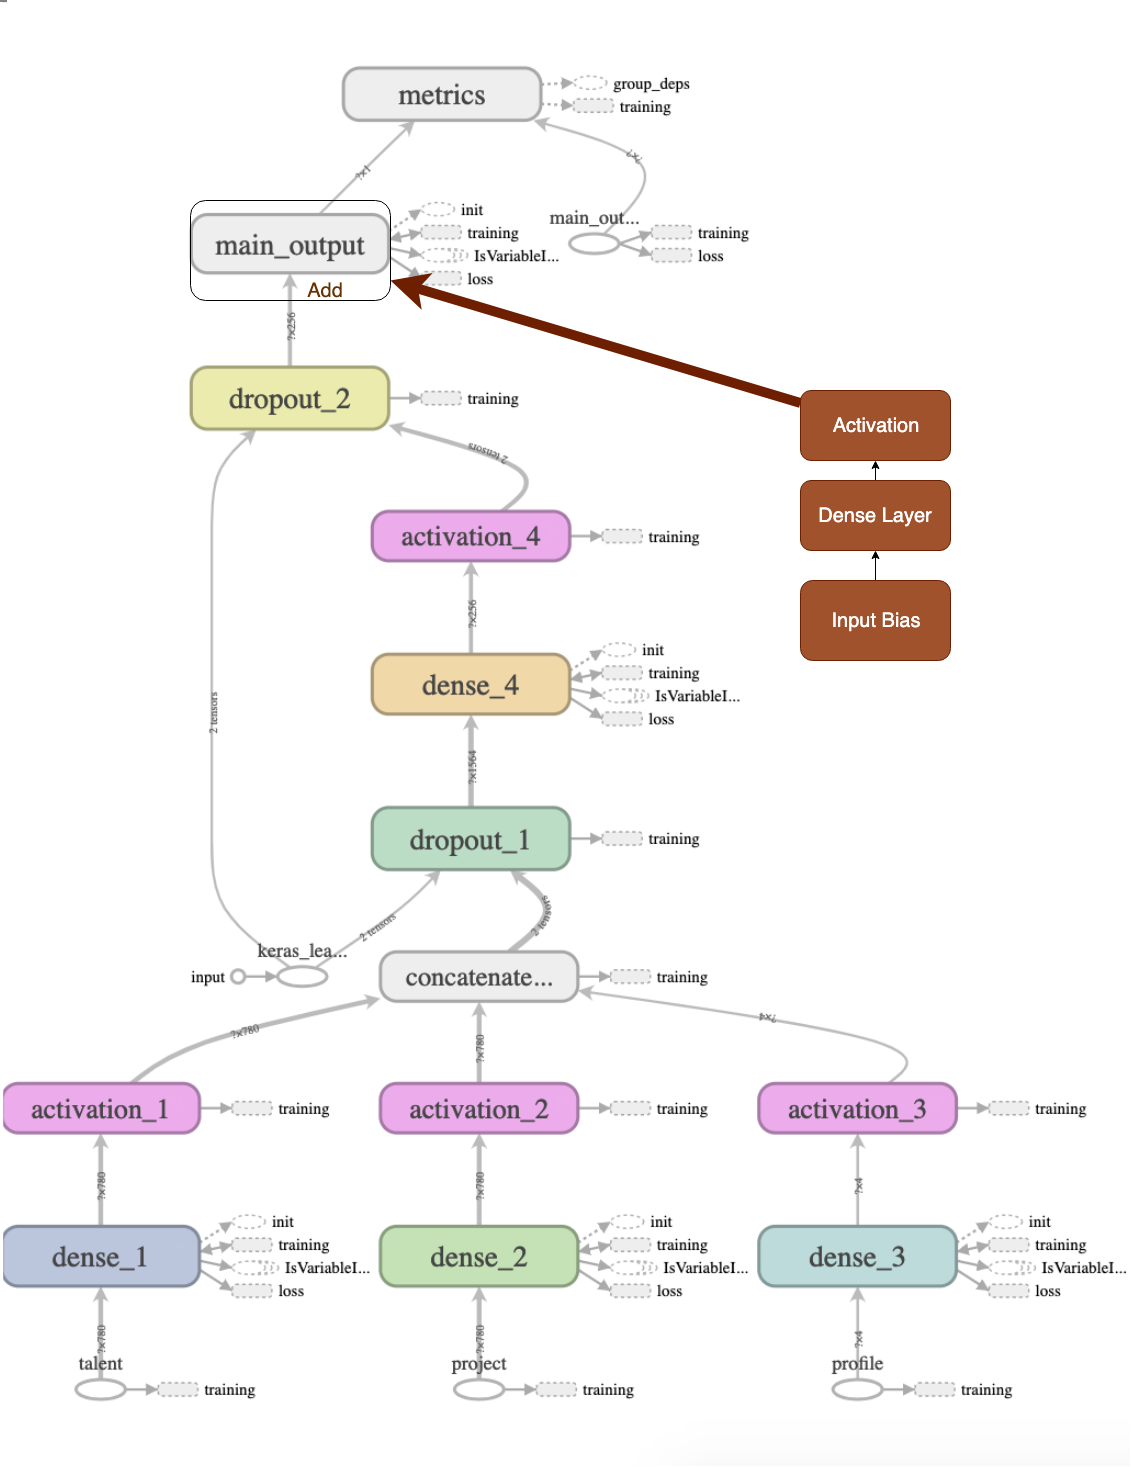
\includegraphics[scale=0.15]{images/TensorBoardFeedback} 
	\caption{Neural networks model with the addition of feedback loop bias}
\end{figure}
\end{frame}
% MSE cost function

\subsection{Group Recommenders} 
\begin{frame}
\frametitle{Group Recommenders}
\begin{itemize}
	\item Group Recommendation using Clustering
	\begin{figure}
		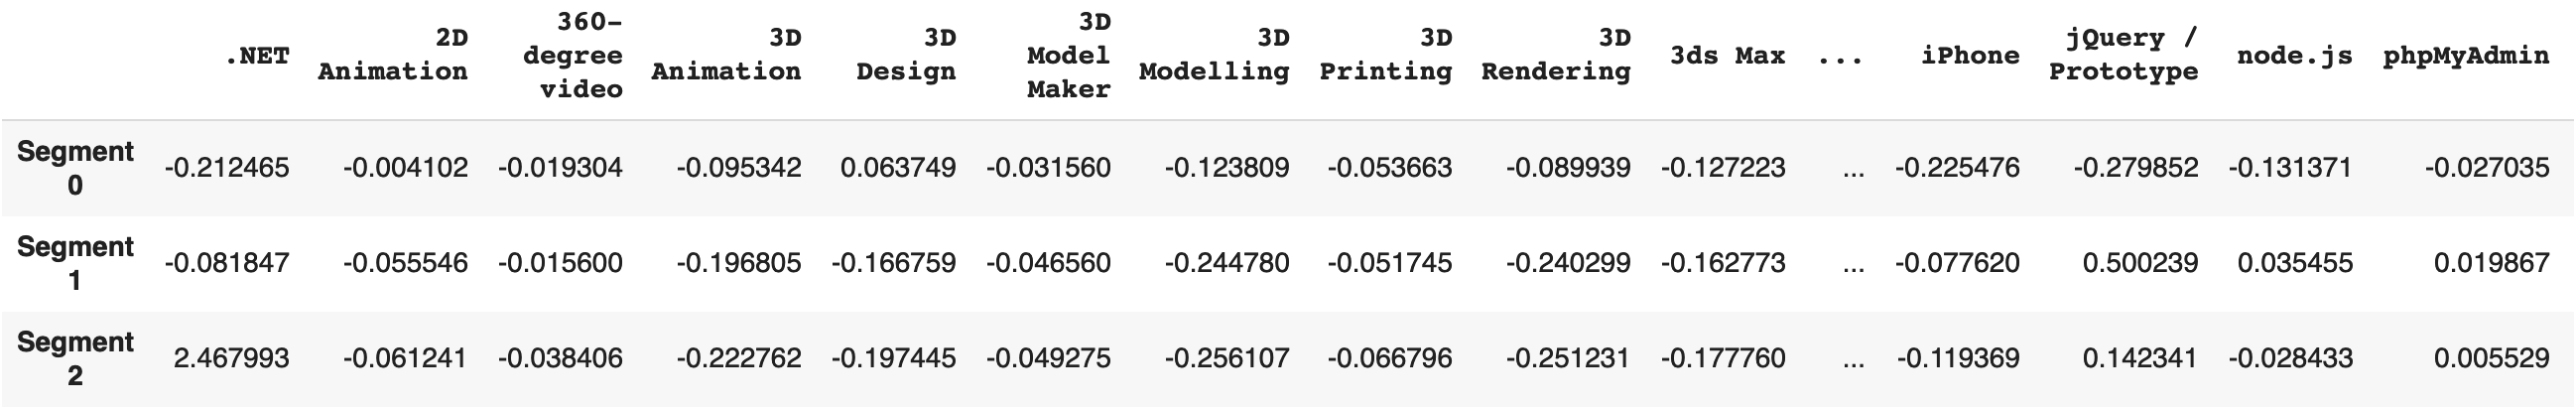
\includegraphics[scale=0.2]{images/ClusterCentersMatrix} 
		\caption{Examples of some centers of clusters that are projected on a 2D space}
	\end{figure}
	\item Unsupervised Group Recommender
	\item Supervised Group Recommender
\end{itemize} 
\end{frame}


\subsection{Unsupervised and Supervised Group Recommender} 
\begin{frame}
\frametitle{Unsupervised and Supervised Group Recommender}
   \begin{itemize}
	\item Baseline Recommender
	\item Diverse Recommender
	\begin{equation}
	g ( R , \lambda ) = ( 1 - \lambda ) \frac { 1 } { | R | } \sum _ { i \in R } f _ { r e l } ( i ) + \lambda d i v ( R ) .
	\label{eq:diversity-equation}
	\end{equation}
\end{itemize} 
   \begin{block}{Diversity Enhancement Algorithm}
	Find the best talent for every role of the project with the equation.
\end{block}
\end{frame}




\subsection{Dashboard Main} 
\begin{frame}
\frametitle{Dashboard Main}
\begin{figure}
	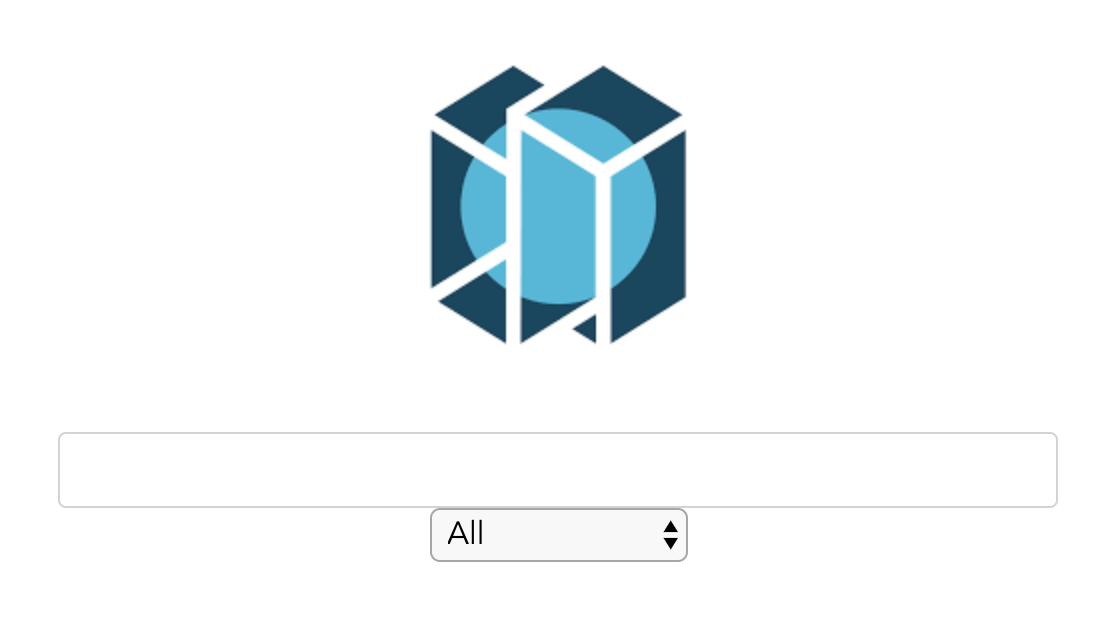
\includegraphics[scale=0.3]{images/DashboardMain} 
	\caption{Main screen of the dashboard}
\end{figure}
\end{frame}

\subsection{Dashboard Projects} 
\begin{frame}
\frametitle{Dashboard Projects}
\begin{figure}
	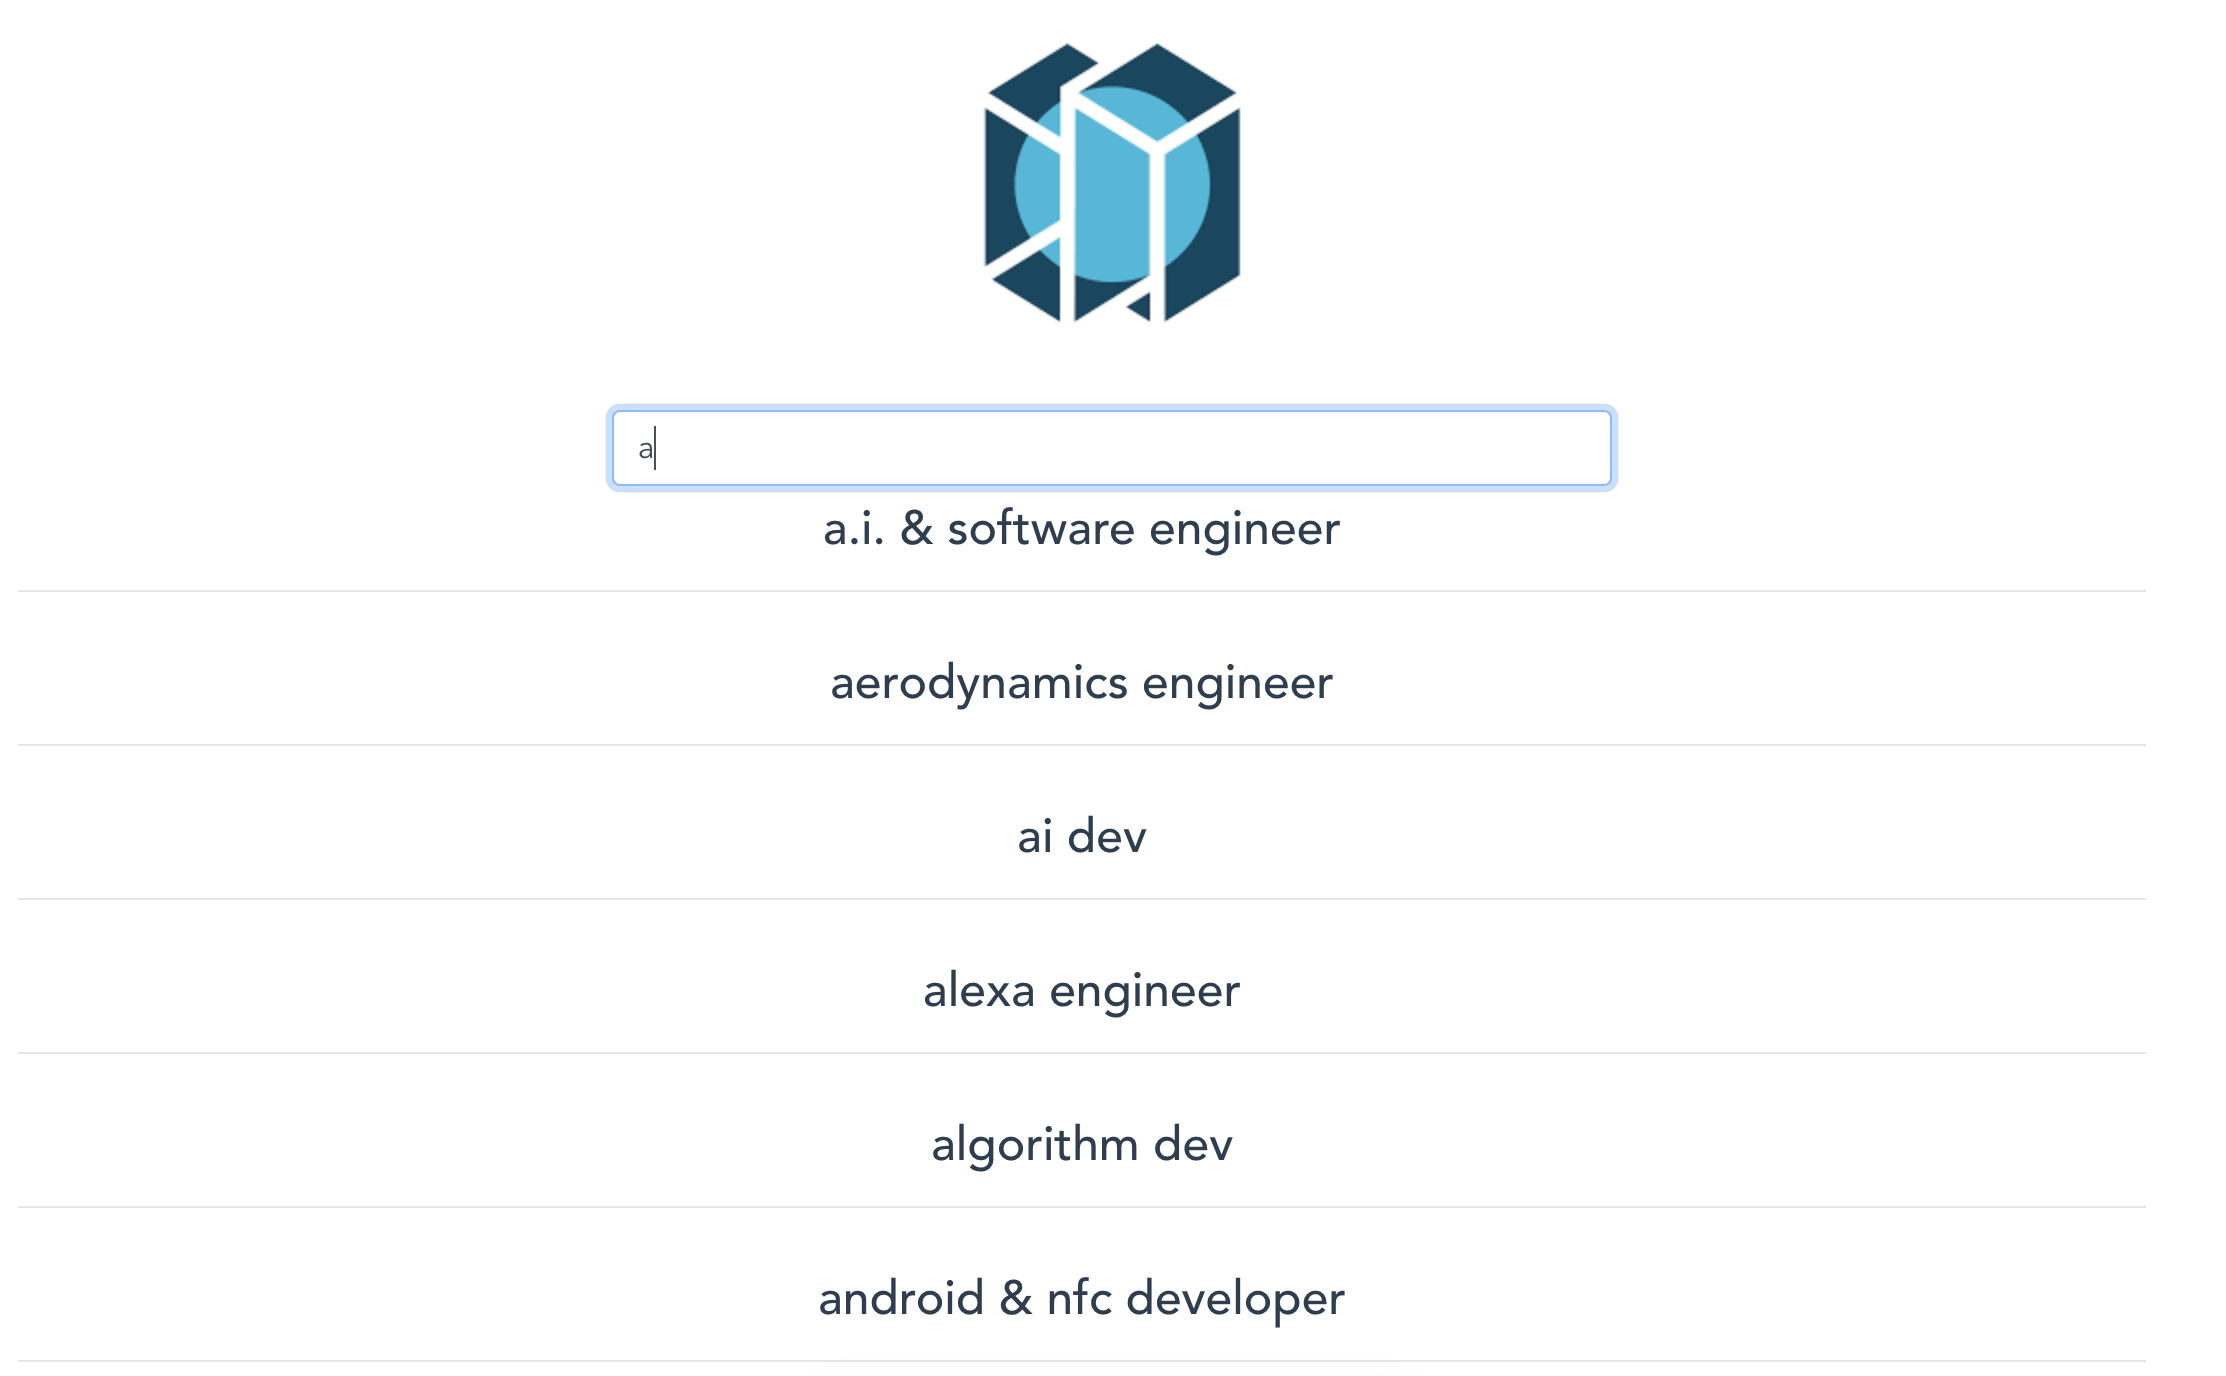
\includegraphics[scale=0.25]{images/DashboardProjects} 
	\caption{A snippet from the list of all projects that start with the letter \textit{a}}
\end{figure}
\end{frame}

\subsection{Dashboard Individual} 
\begin{frame}
\frametitle{Dashboard Individual}
\begin{figure}
	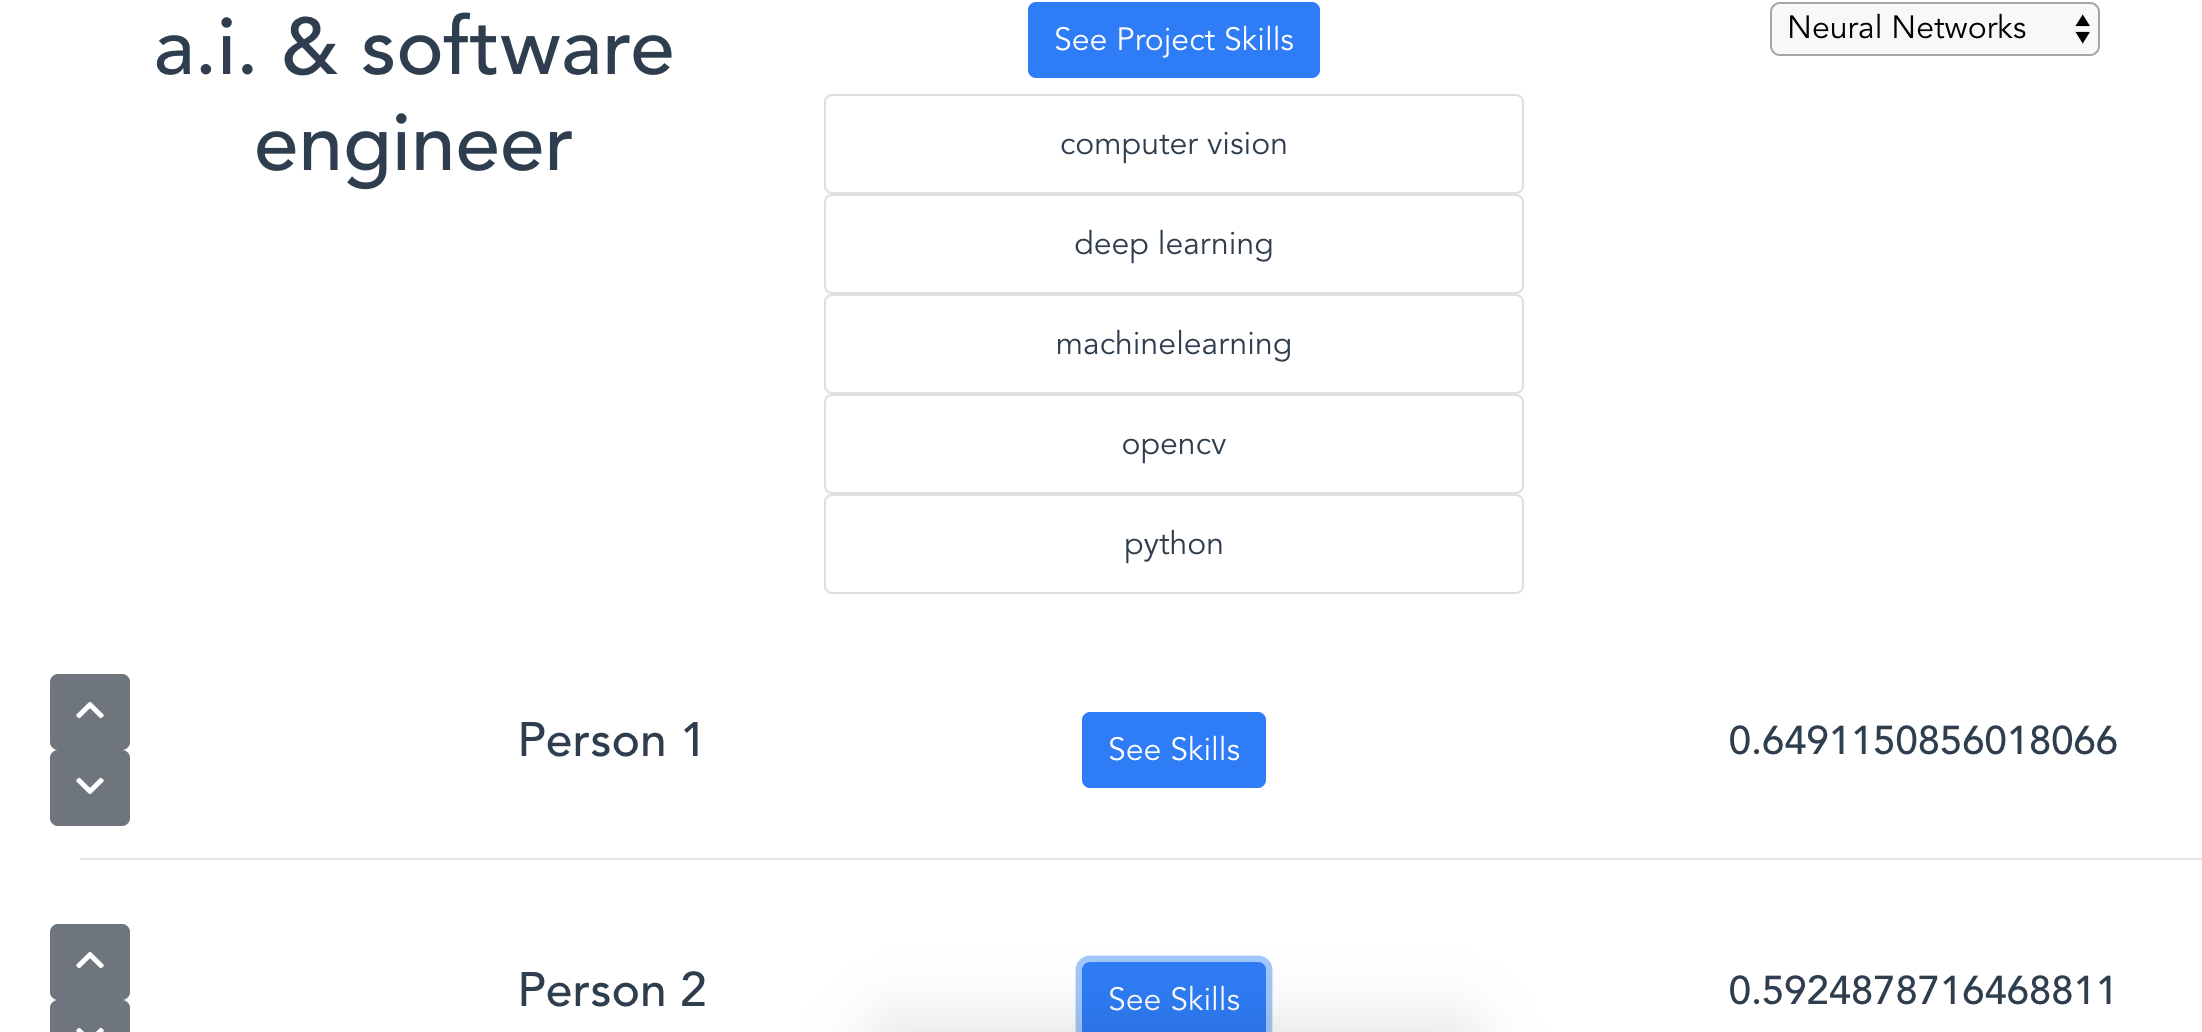
\includegraphics[scale=0.3]{images/DashboardIndividual} 
	\caption{A screenshot from the list of all recommendations from neural networks for the project \textit{a.i. \& software engineer}}
	\end{figure}
\end{frame}

\subsection{Dashboard Individual Hybrid} 
\begin{frame}
\frametitle{Dashboard Individual Hybrid}
\begin{figure}
	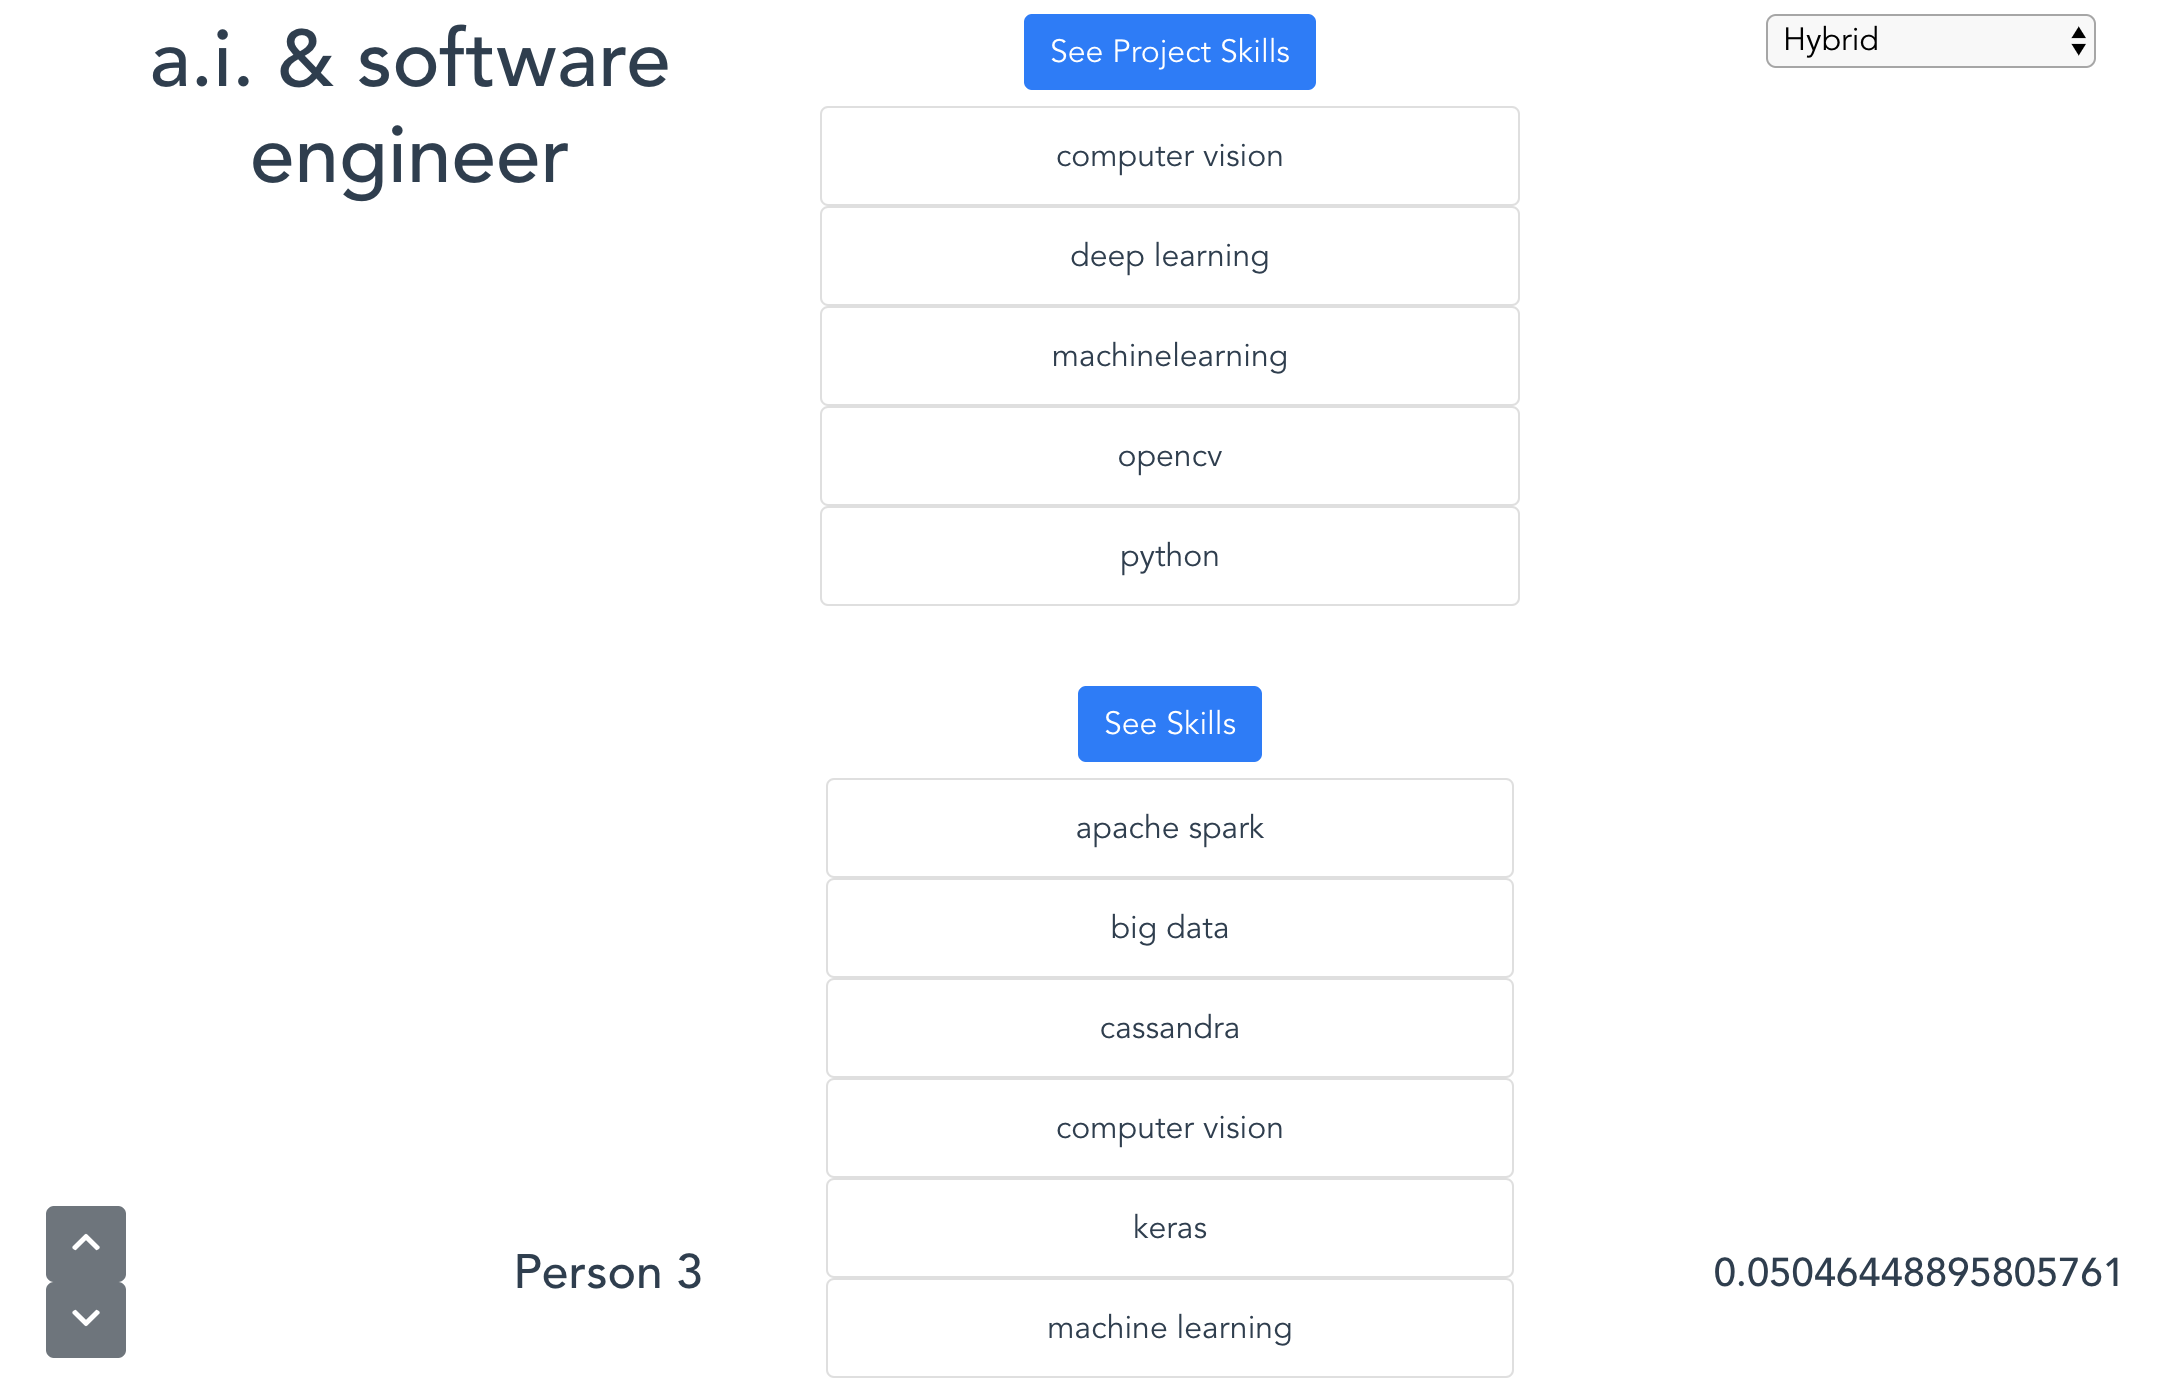
\includegraphics[scale=0.25]{images/DashboardIndividualHybrid} 
	\caption{A screenshot from the list of all recommendations from neural networks for the project \textit{a.i. \& software engineer}}
	\end{figure}
\end{frame}

\subsection{Dashboard Group} 
\begin{frame}
\frametitle{Dashboard Group}
\begin{figure}
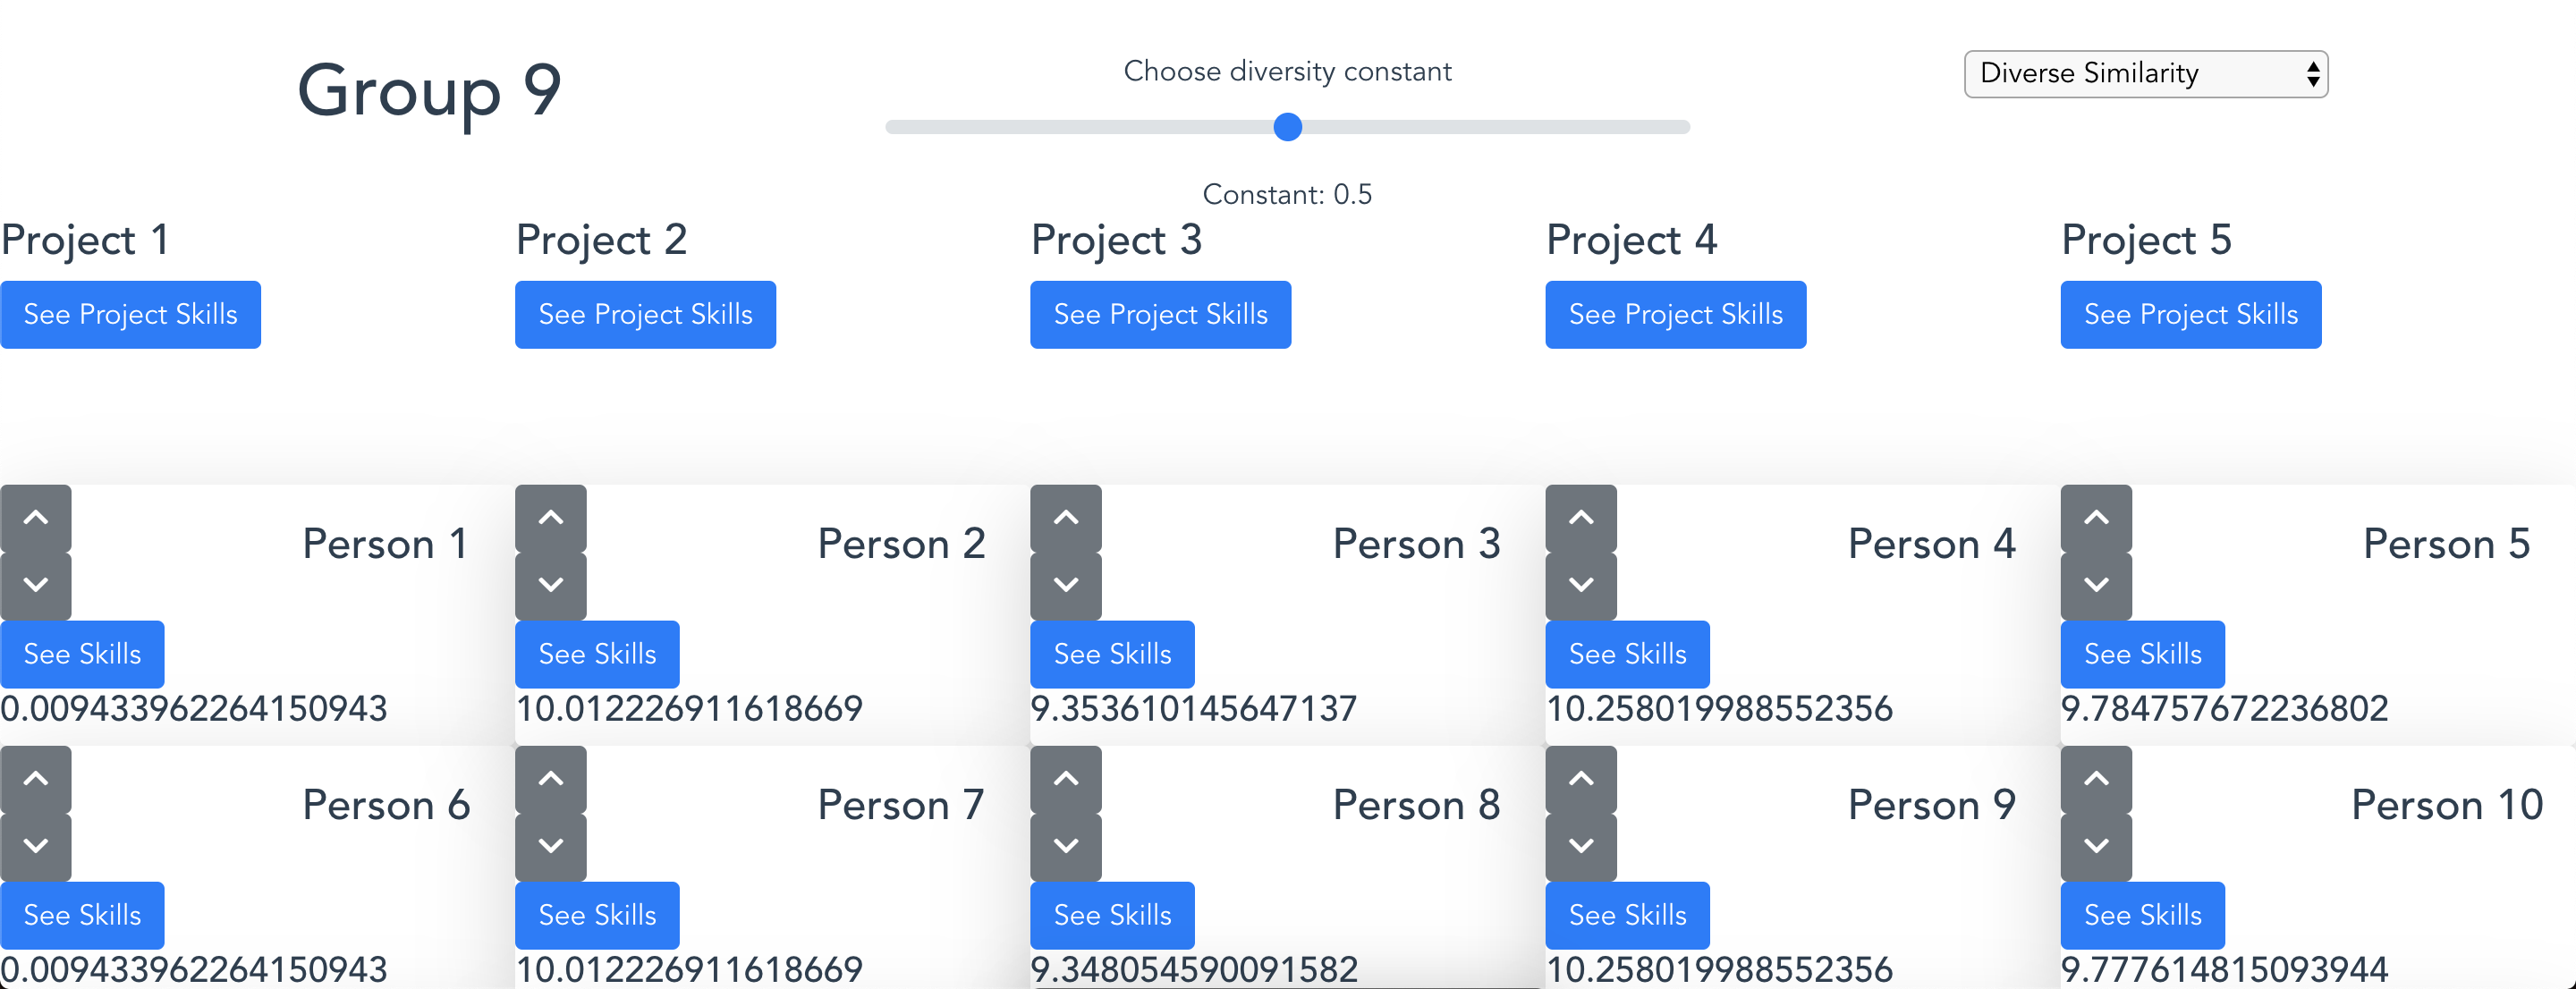
\includegraphics[scale=0.22]{images/DashboardGroup} 
\caption{A screenshot from the list of all recommendations from diverse cosine similarity for the group 9}
\end{figure}
\end{frame}

\section{Evaluation} 
\begin{frame}
\frametitle{Evaluation Methods}
\begin{itemize}
	\item Offline evaluation: evaluation using algorithms
	\item Online evaluation: letting users interact with system and analyzing results
	\item User studies: asking users questions without giving them information about your aim etc.
\end{itemize} 
\end{frame}

\subsection{Offline Accuracy of Individual Recommenders} 
\begin{frame}
   \frametitle{Offline Accuracy of Individual Recommenders}
\begin{table}[htp]
	\caption{Offline evaluation results for different recommenders are shown.}
	\centering
	\begin{tabular}{|l|l|l|l|}
		\hline
		Type         & Name           & Top 1 & Top 5 \\ \hline
		Unsupervised & Motius         & 0.07  & 0.21  \\ \hline
		Unsupervised & Similarity     & 0.28  & 0.36  \\ \hline
		Unsupervised & Popularity     & 0.07  & 0.45  \\ \hline
		Unsupervised & Similarity\&Popularity         & 0.12  & 0.29  \\ \hline
		Supervised   & Neural Network & 0.19  & 0.56  \\ \hline
		Supervised   & Neural Network \& Similarity & 0.1  & 0.49  \\ \hline
	\end{tabular}
	\label{discussion:accuracy-offline}
\end{table}
\end{frame}

\subsection{User Study Results of Individual Recommenders} 
\begin{frame}
\frametitle{User Study Result of Individual Recommenders}
\begin{table}[htp]
	\caption{Offline evaluation results for different recommenders are shown.}
	\centering
	\begin{tabular}{|l|l|l|l|}
		\hline
		Type         & Name           & First Item Value & Satisfaction \\ \hline
		Unsupervised & Similarity     & 4.375  & 3.8125  \\ \hline
		Supervised   & Neural Network & 2.5625  & 2.8125  \\ \hline
		Supervised   & Hybrid & 4.5  & 4.0625  \\ \hline
	\end{tabular}
	\label{discussion:accuracy-offline}
\end{table}
\end{frame}

\subsection{Accuracy of Unsupervised Group Recommender} 
\begin{frame}
\frametitle{Accuracy of Unsupervised Group Recommender}
\begin{figure}
	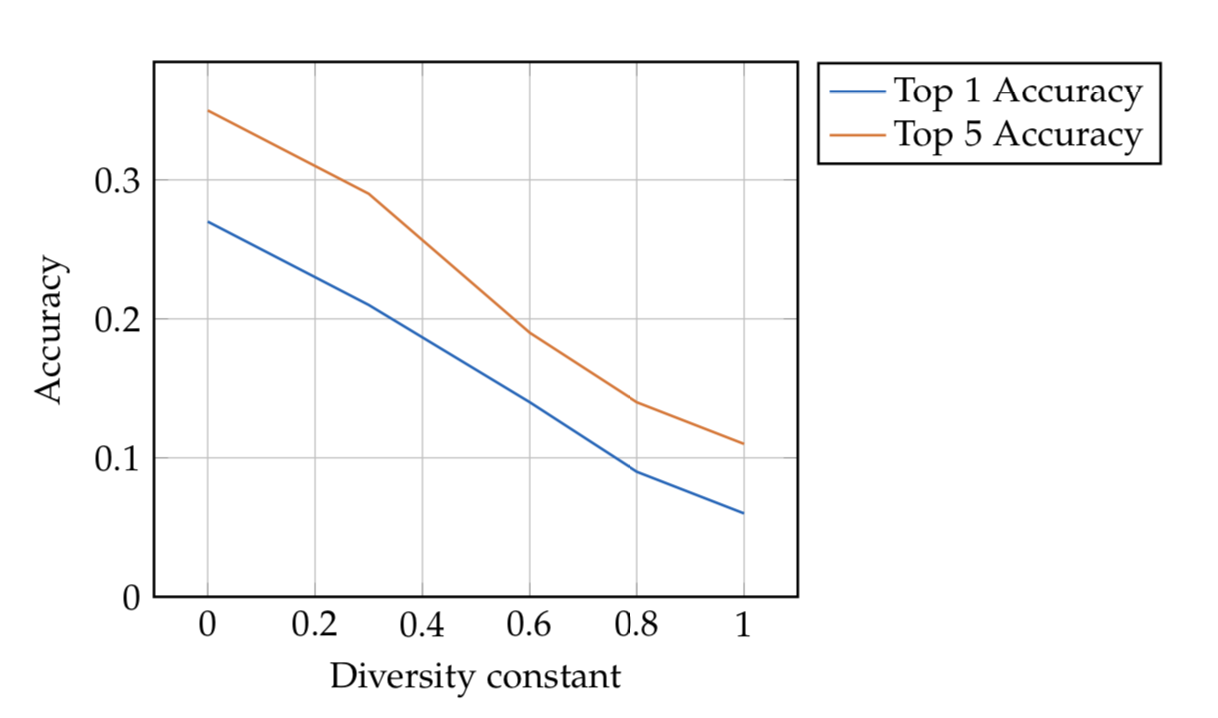
\includegraphics[scale=0.4]{images/diversity-unsupervised-group-accuracy} 
	\caption{Effect of diversity constant on unsupervised group recommender to the accuracy}
\end{figure}
\end{frame}

\subsection{Diversity of Unsupervised Group Recommender} 
\begin{frame}
\frametitle{Accuracy of Unsupervised Group Recommender}
\begin{figure}
	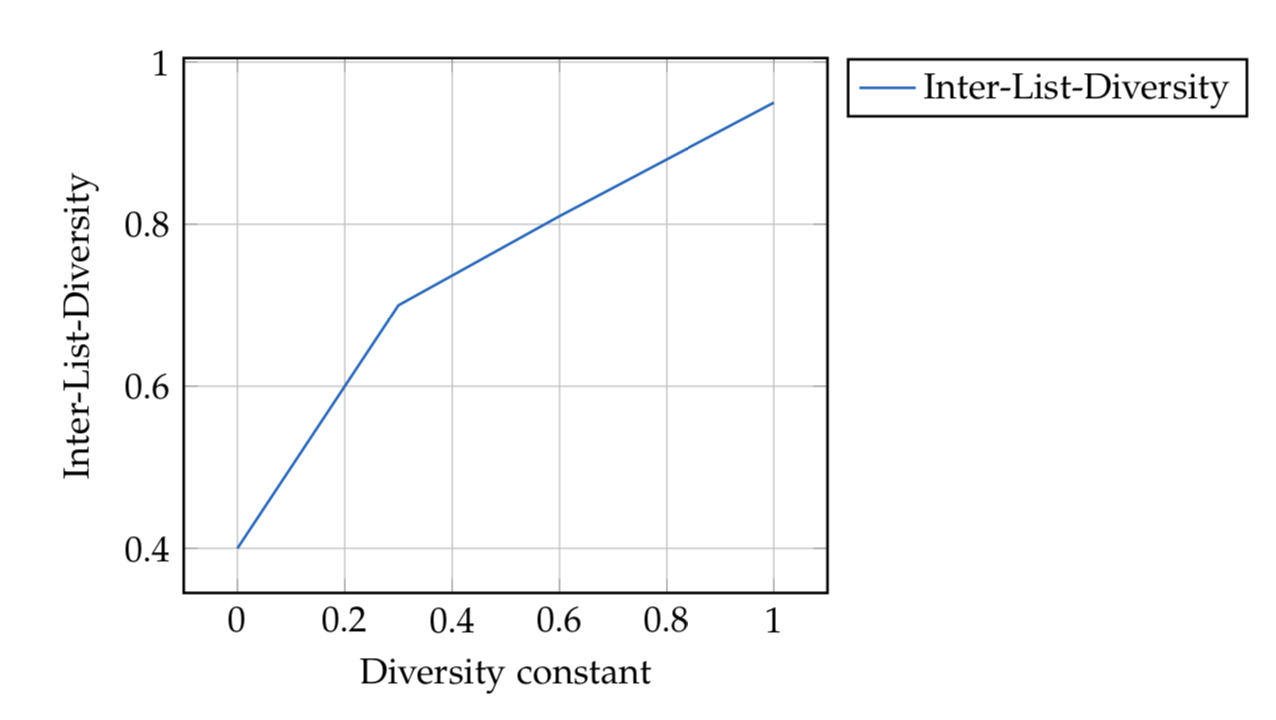
\includegraphics[scale=0.4]{images/unsupervised-group-diversity} 
	\caption{Effect of diversity constant on unsupervised group recommender to the diversity}
\end{figure}
\end{frame}

\subsection{User Study about Unsupervised Group Recommender} 
\begin{frame}
\frametitle{User Study about Unsupervised Group Recommender}
\begin{figure}
	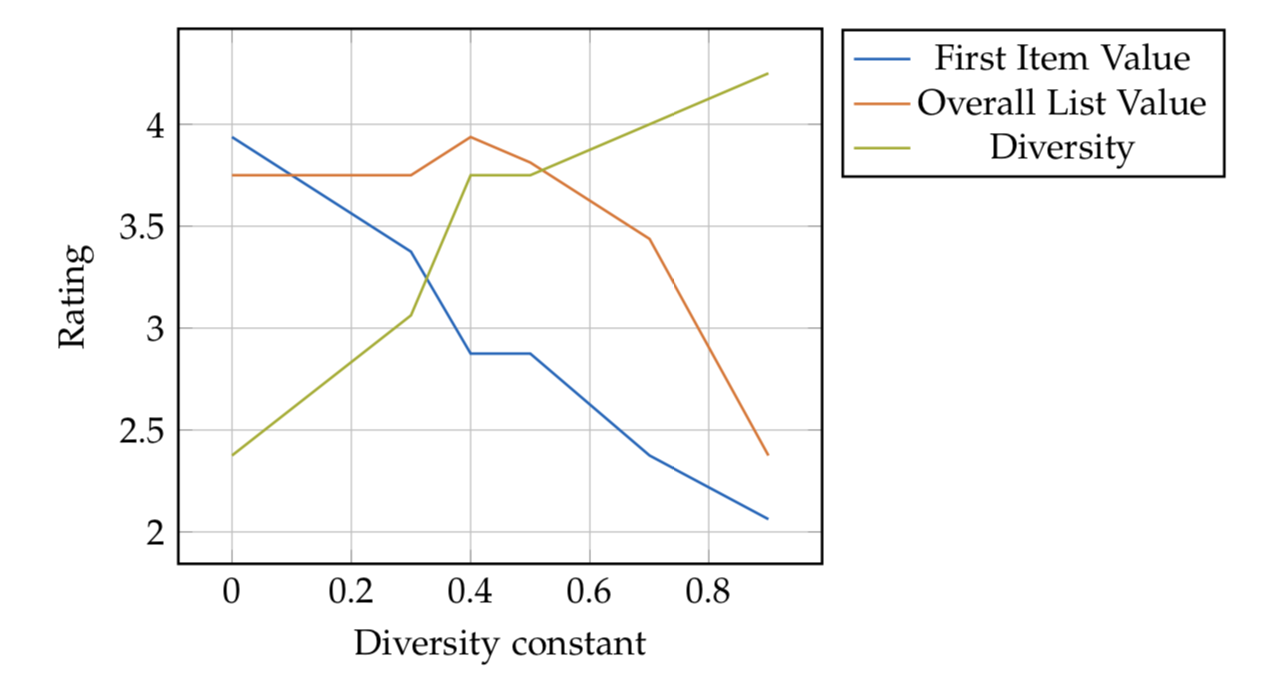
\includegraphics[scale=0.4]{images/diversity-unsupervised-group-user-study} 
	\caption{Effect of diversity constant on unsupervised group recommender to the average user opinion}
\end{figure}
\end{frame}

% Down: supervised
\subsection{Accuracy of Supervised Group Recommender} 
\begin{frame}
\frametitle{Accuracy of Supervised Group Recommender}
\begin{figure}
	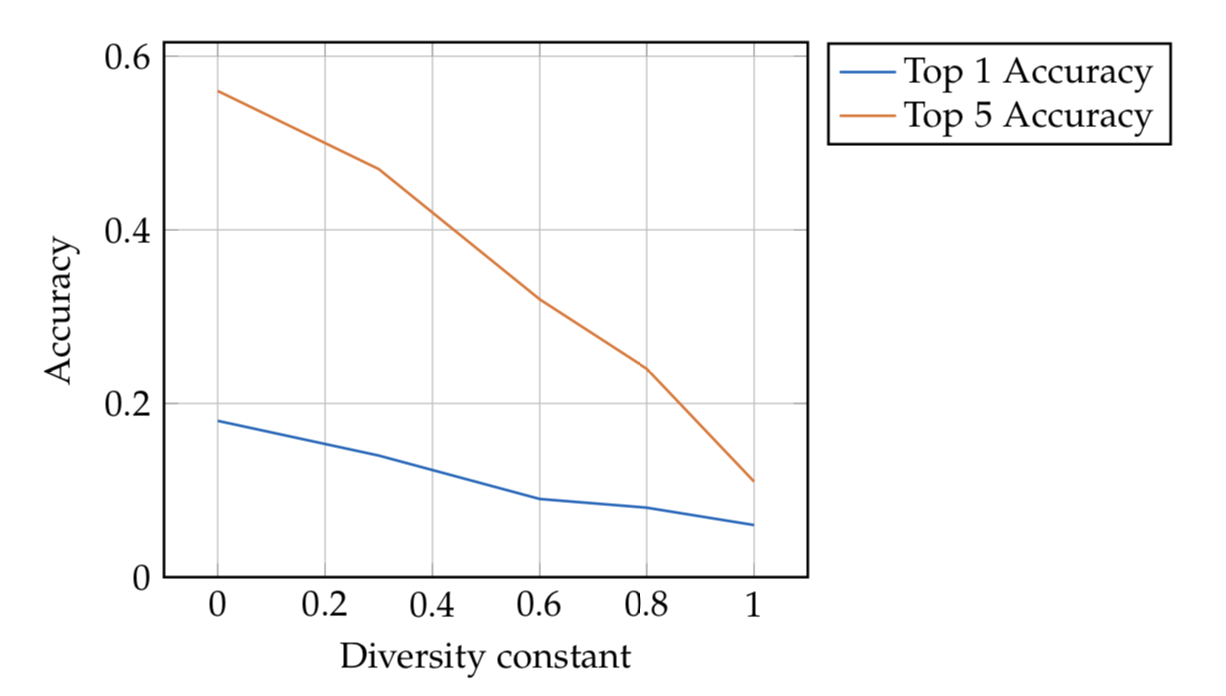
\includegraphics[scale=0.4]{images/supervised-group-accuracy} 
	\caption{Effect of diversity constant on supervised group recommender to the accuracy}
\end{figure}
\end{frame}

\subsection{Diversity of Supervised Group Recommender} 
\begin{frame}
\frametitle{Accuracy of Supervised Group Recommender}
\begin{figure}
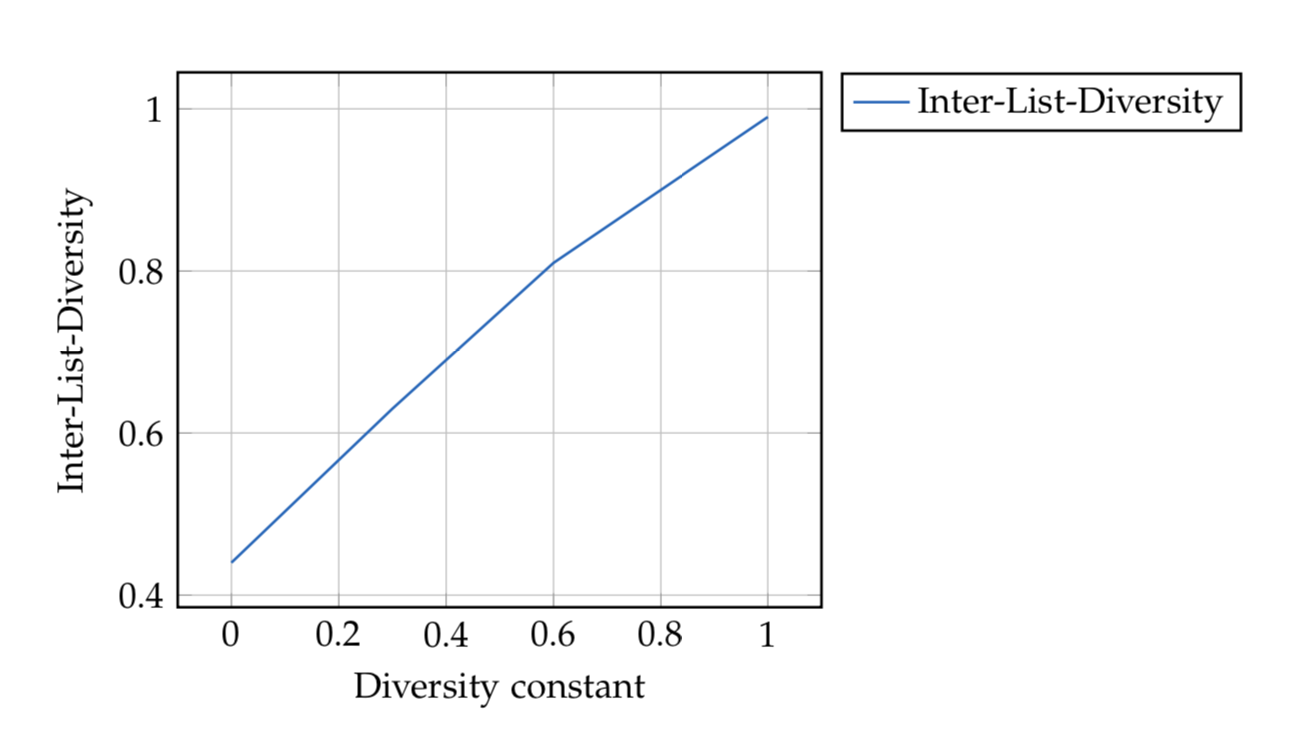
\includegraphics[scale=0.4]{images/supervised-group-diversity} 
\caption{Effect of diversity constant on supervised group recommender to the diversity}
\end{figure}
\end{frame}

\subsection{User Study about Supervised Group Recommender} 
\begin{frame}
\frametitle{User Study about Supervised Group Recommender}
\begin{figure}
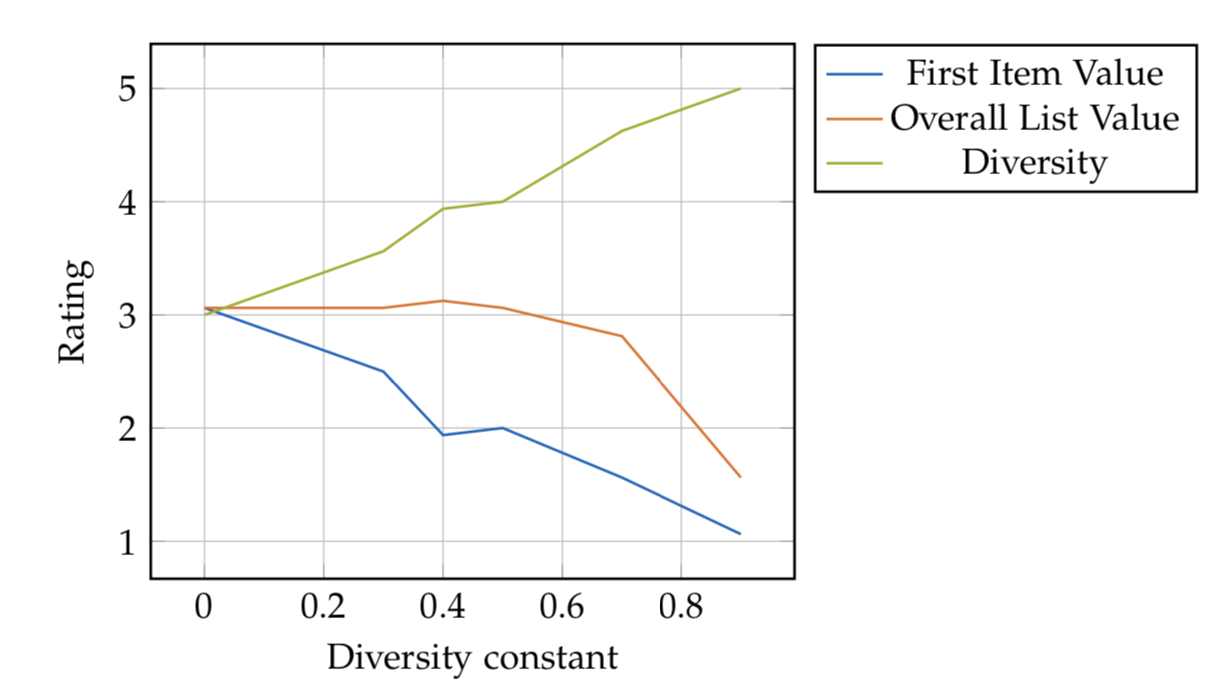
\includegraphics[scale=0.4]{images/supervised-group-user} 
\caption{Effect of diversity constant on supervised group recommender to the average user opinion}
\end{figure}
\end{frame}

\subsection{Online Evaluation and User Study about Feedback Learning} 
\begin{frame}
\frametitle{Online Evaluation and User Study about Feedback Learning}
\begin{table}[htp]
	\caption[Online Evaluation Table]{A table that shows the user opinions before and after re-training.}
	\centering
	\begin{tabular}{|l|l|l|}
		First Item Value & Overall List Value & Diversity \\
		3.125 & 3 & 2.375\\
		3.75 & 3.6875 & 2.5625 \\
	\end{tabular}
\end{table}
\end{frame}

\section{Conclusion} 
\begin{frame}
\frametitle{Conclusion}
Initial questions:
\begin{itemize}
	\item Does high accuracy guarantee high user satisfaction?
	\item Does diversity affect user satisfaction positively?
	\item Would a feedback loop enhance user satisfaction?
\end{itemize} 
Answers:
\begin{itemize}
	\item No, we proved otherwise.
	\item Yes from our experiments. However, more experiments with more subjects are needed.
	\item Yes, if there are enough feedback.
\end{itemize} 
\end{frame}

\subsection{Artificial Neural Networks} 
\begin{frame}
\frametitle{Artificial Neural Networks}

\begin{figure}
	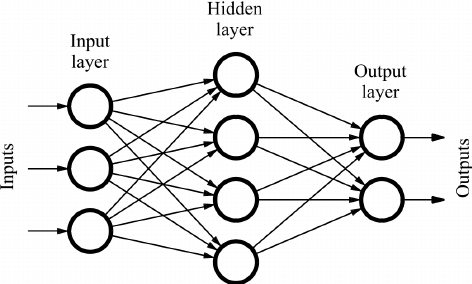
\includegraphics[scale=0.3]{images/FFNN} 
	\caption{High level architecture of a feedforward neural network}
\end{figure}

\begin{equation}
f(\boldsymbol{x} ; \boldsymbol{w}, b)=\sigma(\boldsymbol{x}^{\top} \boldsymbol{w}+b)
\label{eq:nn-one-layer}
\end{equation} 

\begin{block}{Embeddings}
	Embeddings layers are used to reduce dimensionality.
\end{block}

\end{frame}

\subsection{Others Evaluation Methods} 
\begin{frame}
\frametitle{Others Evaluation Methods}

\begin{equation}
\mathrm { ILD } = \frac { 1 } { | R | ( | R | - 1 ) } \sum _ { i \in R } \sum _ { j \in R } d ( i , j ) .
\label{eq:ild}
\end{equation}

\begin{equation}
\mathrm {Unexp} = \frac { 1 } { | R | \left| \mathcal { J } _ { u } \right| } \sum _ { i \in R } \sum _ { j \in \mathcal { J } _ { u } } d ( i , j ) ,
\label{eq:unexp}
\end{equation}


where 

\begin{equation}
\mathcal { J } _ { u } \stackrel { \mathrm { def } } { = } \{ i \in \mathcal { J } | r ( u , i ) \neq \emptyset \} .
\label{eq:unexp-set}
\end{equation}



\end{frame}


\subsection{Freelancer.com Dataset(1)} 
\begin{frame}
\frametitle{Freelancer.com Dataset(1)}

\begin{figure}
	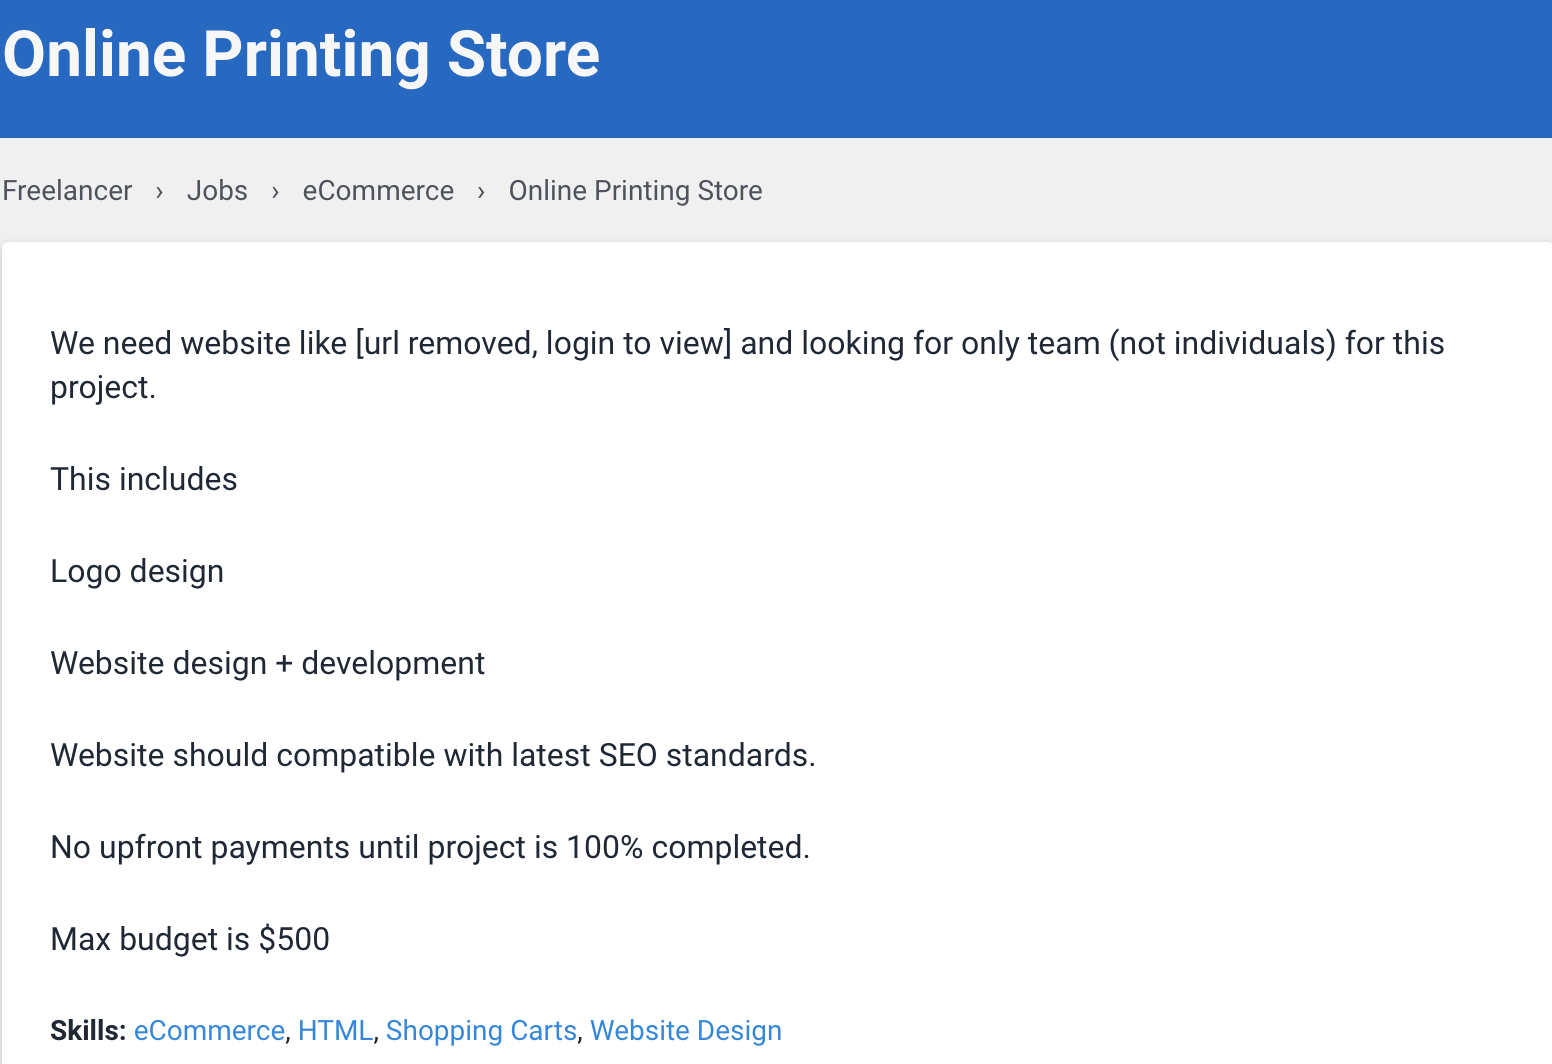
\includegraphics[scale=0.3]{images/FreelancerExample} 
	\caption{An example project from the Freelancer.com Website}
\end{figure}
\end{frame}

\subsection{Freelancer.com Dataset(2)} 
\begin{frame}
\frametitle{Freelancer.com Dataset(2)}

\begin{figure}
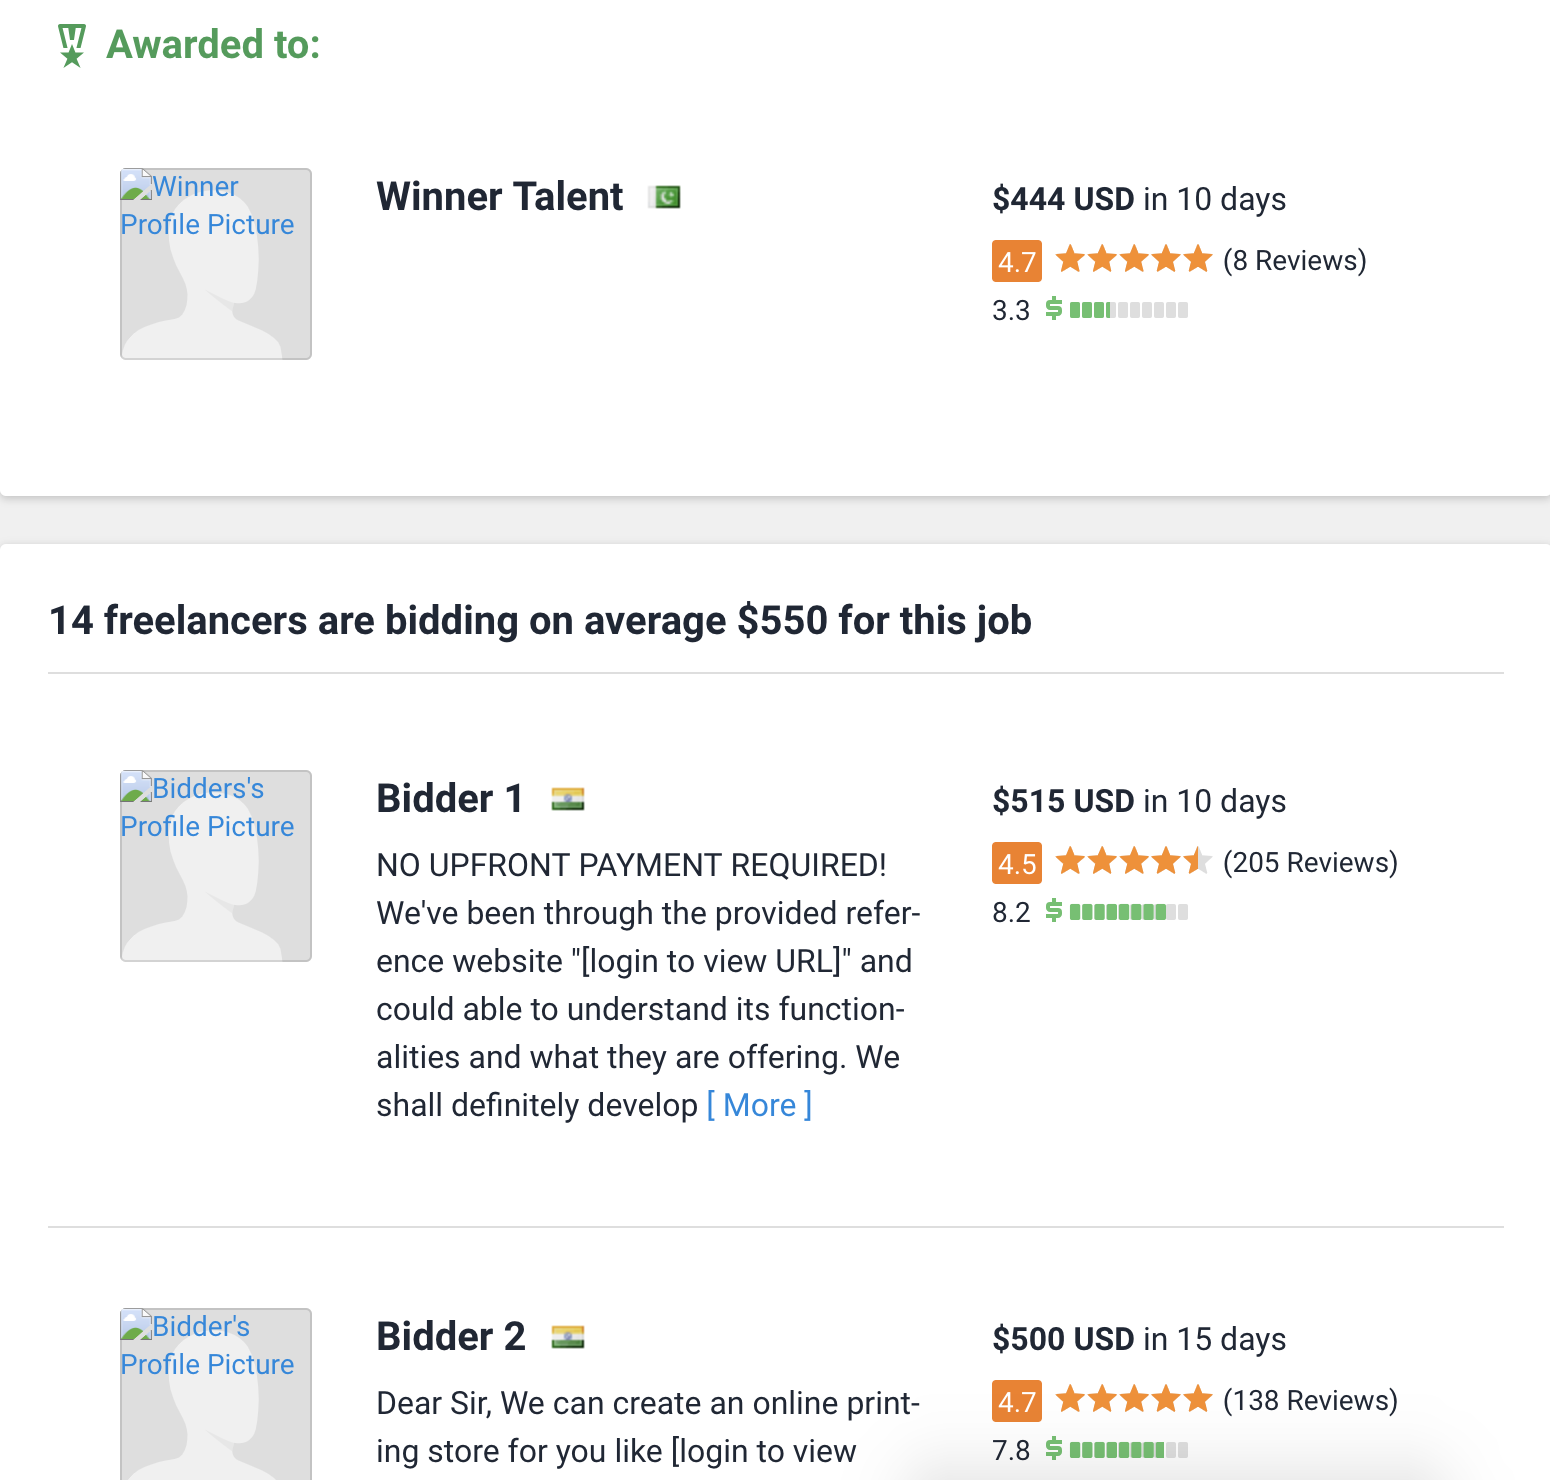
\includegraphics[scale=0.2]{images/FreelancerTalentExample} 
\caption{The winner and other bidders to the same project}
\end{figure}
\end{frame}

\subsection{Freelancer.com Dataset(3)} 
\begin{frame}
\frametitle{Freelancer.com Dataset(3)}

\begin{figure}
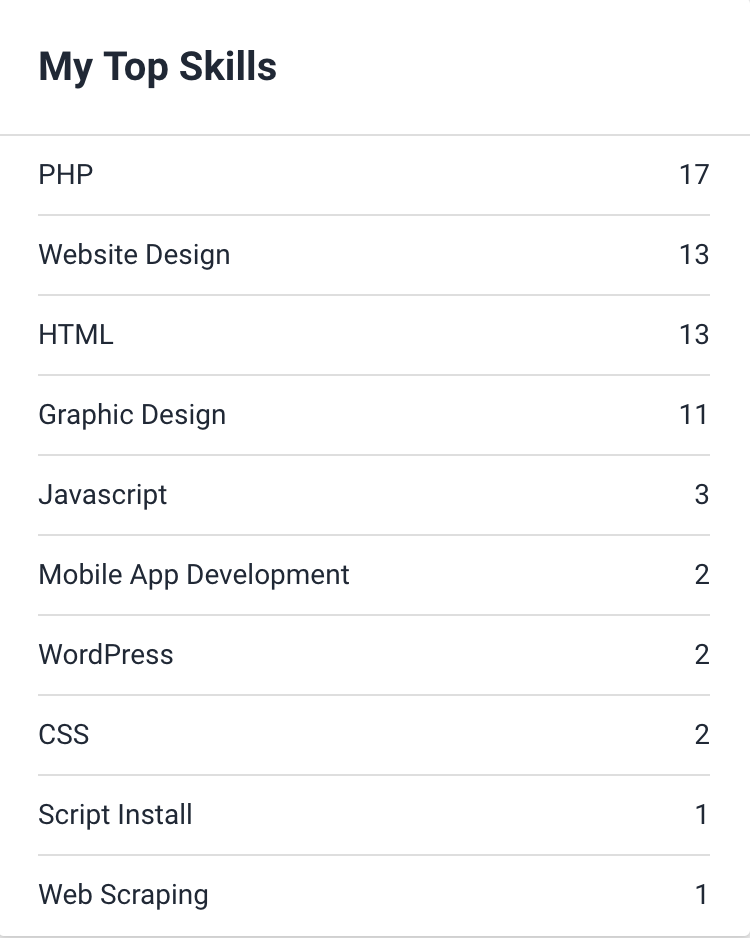
\includegraphics[scale=0.3]{images/FreelancerTalentSkills} 
\caption{The list of tops skills by a talent on Freelancer.com web page}
\end{figure}
\end{frame}

\subsection{Model of Sparse Input} 
\begin{frame}
\frametitle{Model of Sparse Input}
\begin{figure}
	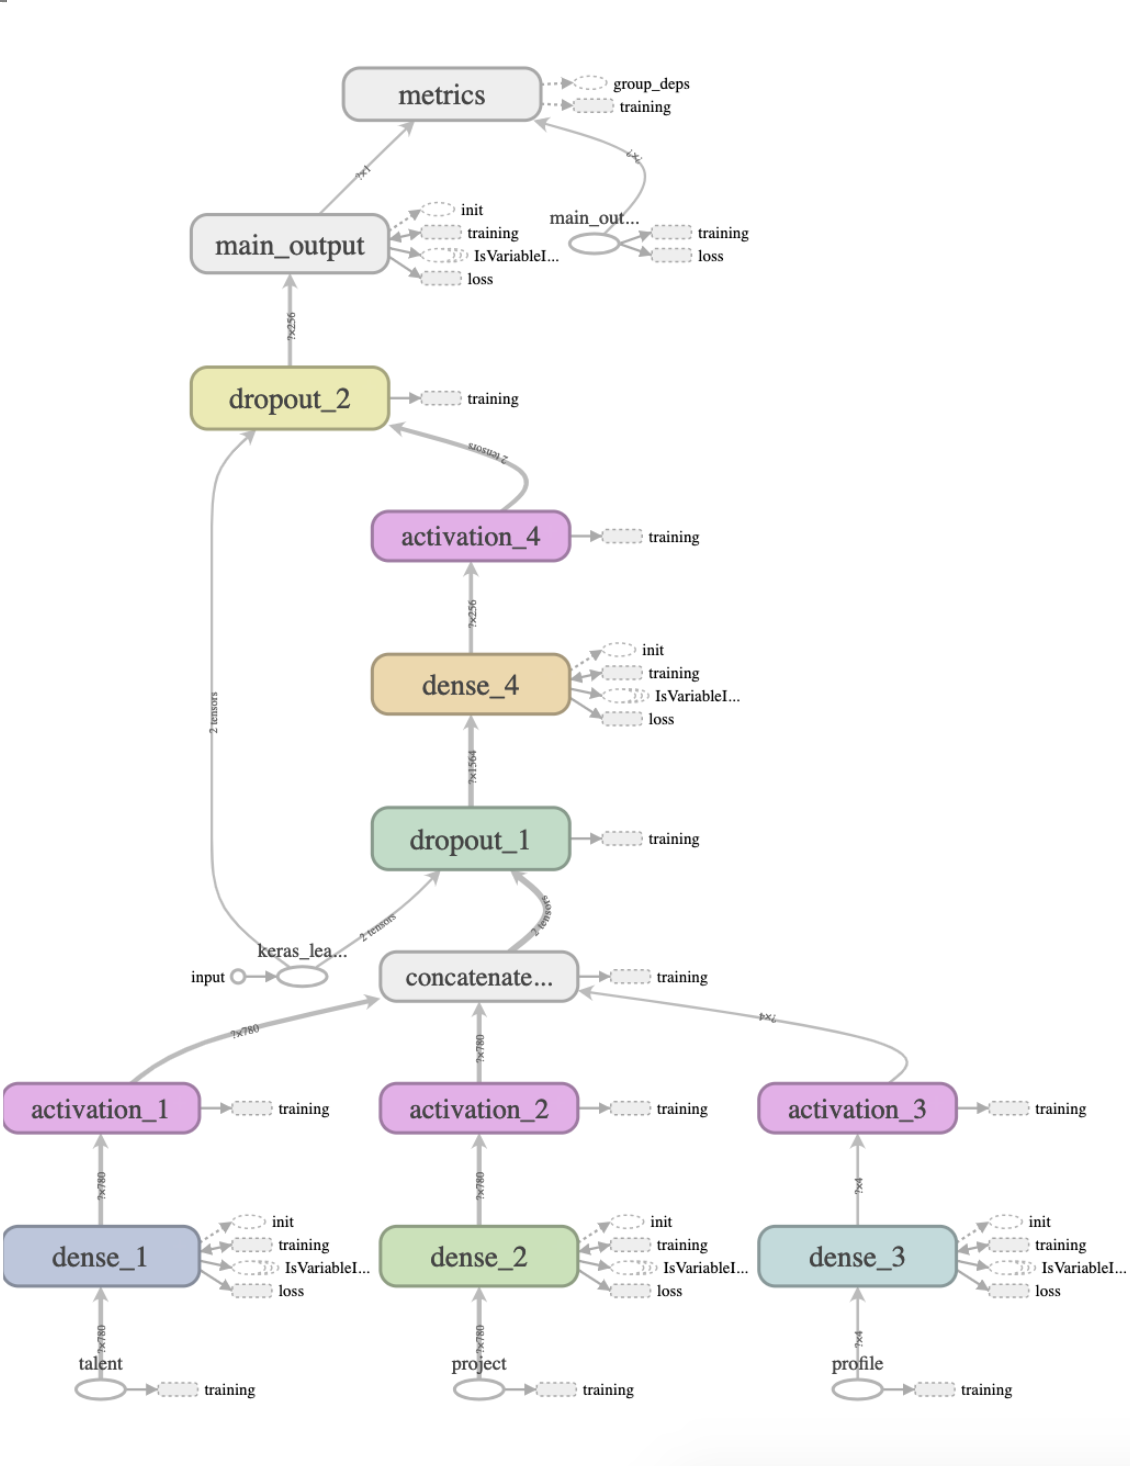
\includegraphics[scale=0.3]{images/TensorBoardSparseCropped} 
	\caption{The graph that explains the sparse input model}
\end{figure}
\end{frame}


\subsection{Supervised Individual Recommender} 
\begin{frame}
\frametitle{Supervised Individual Recommender}
\begin{itemize}
	\item Using Sparse Input
	\begin{figure}
		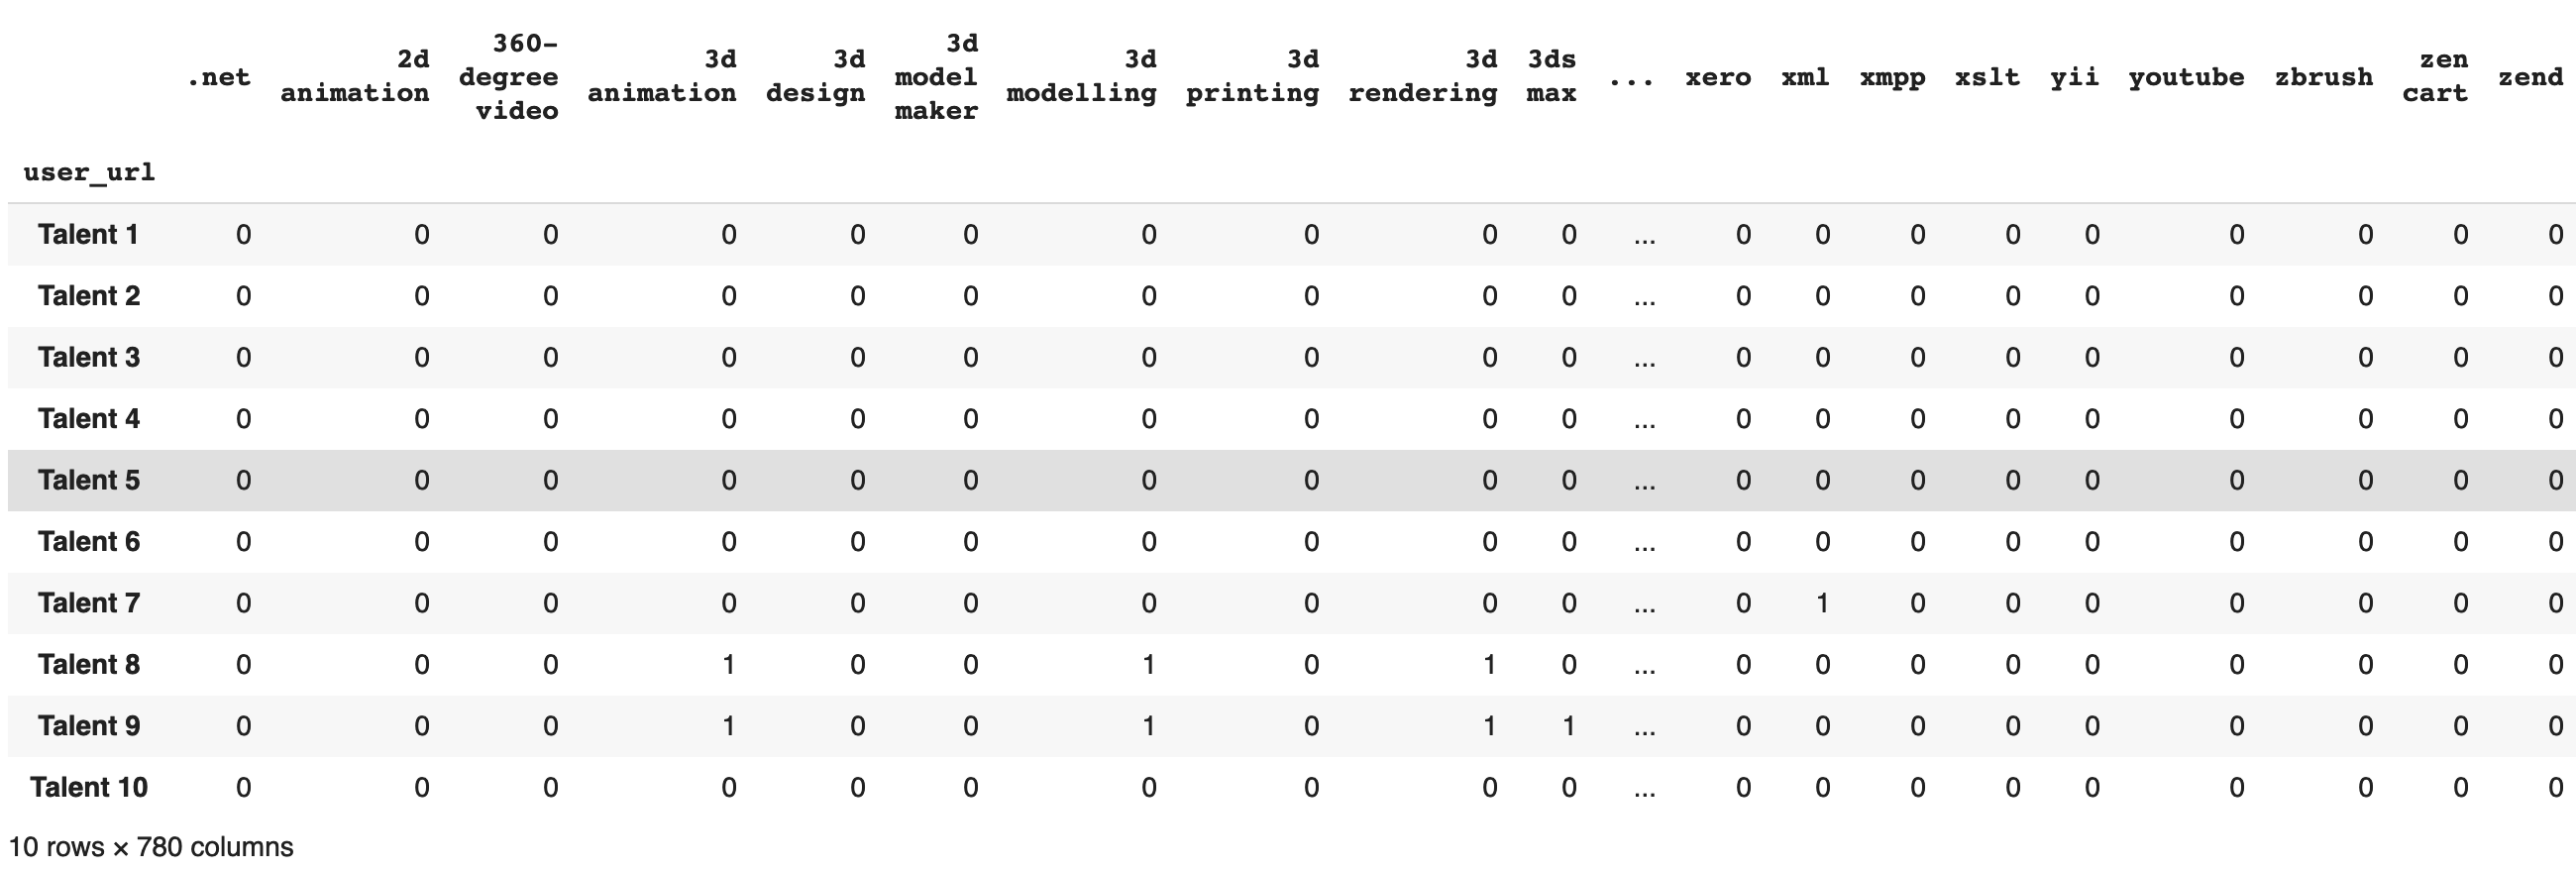
\includegraphics[scale=0.2]{images/FreelancerTalentSkillsMatrix} 
		\caption{The talent skill matrix from freelancer.com}
	\end{figure}
	\item Using Embeddings
	\begin{figure}
		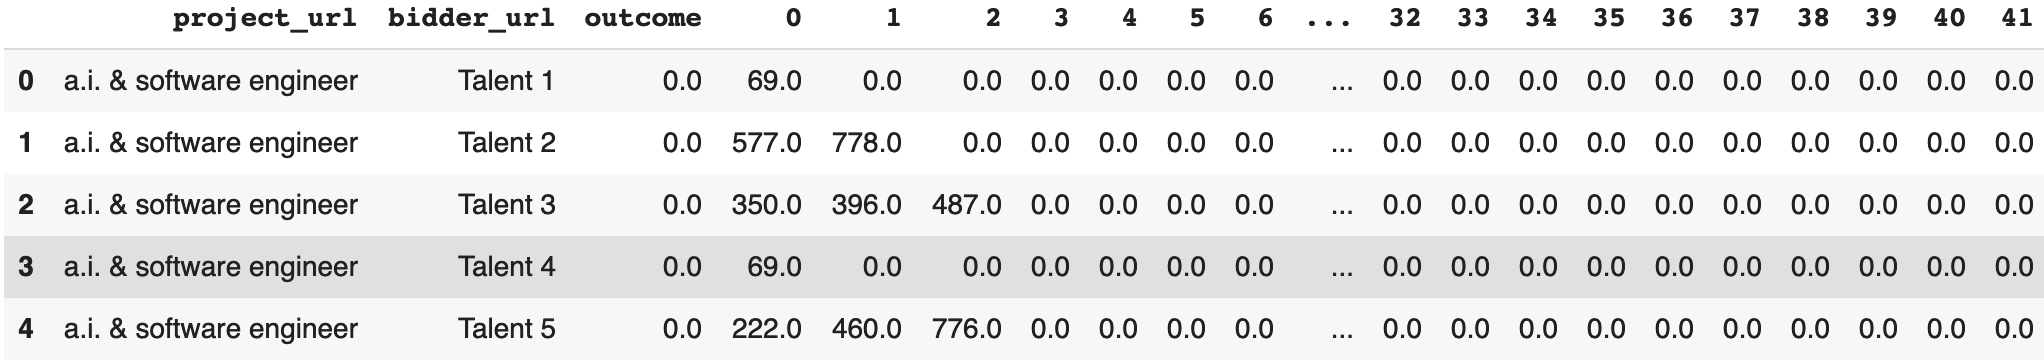
\includegraphics[scale=0.2]{images/EmbeddingTrainingMatrix} 
		\caption{Training data that contains padded embedding skill vectors}
	\end{figure}
\end{itemize} 
\end{frame}

% we use embeddings because memory

\subsection{Extra Information} 
\begin{frame}
\frametitle{Extra Profile Information }
\begin{figure}
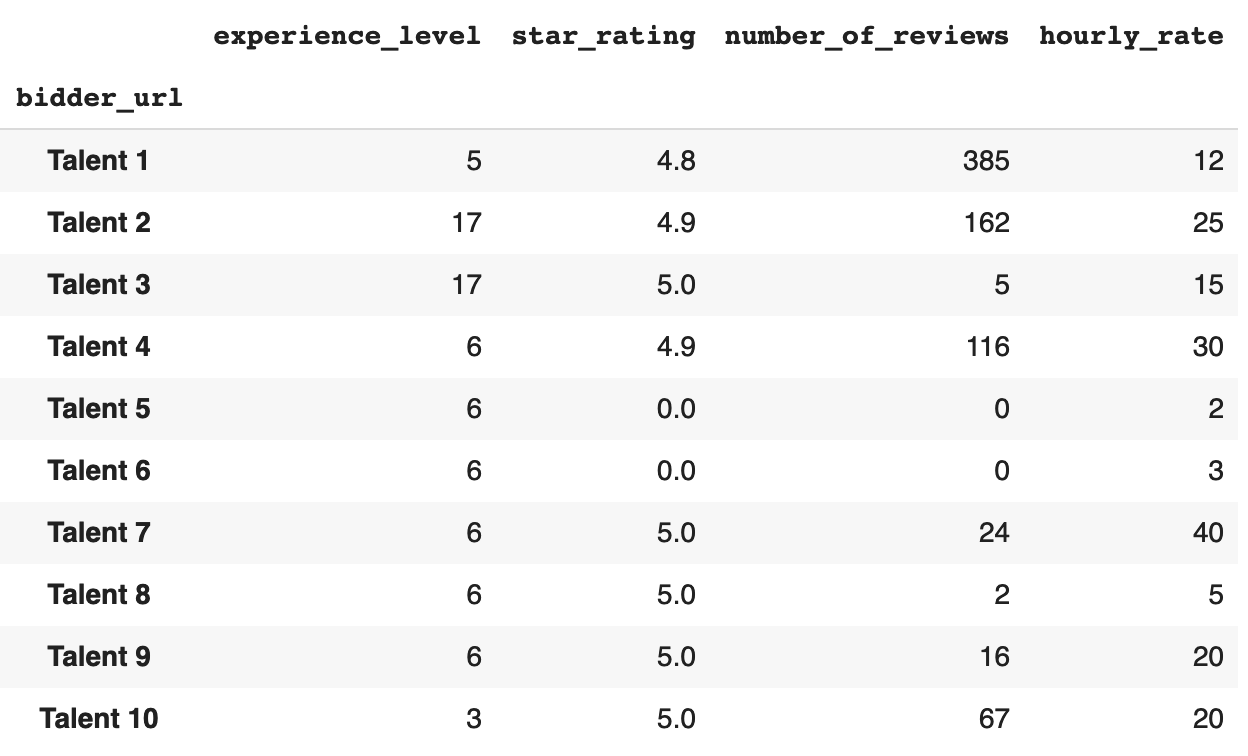
\includegraphics[scale=0.4]{images/FreelancerTalentMeta} 
\caption{The talent extra information matrix from Freelancer.com}
\end{figure}
\end{frame}


\end{document}
